\documentclass[lang=cn,11.9pt,a4paper,cite=authoryear]{elegantpaper}

\title{COVID-19疫情趋势预测研究}
\author{肖世莺 \and 张红丽 \and 成宏媛 \and 王瑜}
\date{}

\usepackage{array}
\newcommand{\ccr}[1]{\makecell{{\color{#1}\rule{1cm}{1cm}}}}
\usepackage{subfigure}

\begin{document}

\maketitle

\begin{abstract}
本文使用SEIR模型和LSTM模型对6个高风险国家的COVID-19疫情预测进行模拟评估,分析了SEIR模
型和LSTM模型预测的准确性,并对COVID-19疫情的峰值和未来5天的累计确诊人数进行预测估计。本
文的目的是帮助理解COVID-19的传播动态,了解目前的疫情发展趋势。如果想要了解本文的相关数
据和程序代码,请访问\href{https://github.com/data-science-in-action/project-stat223}{project-stat223}
。
\keywords{COVID-19,SEIR,LSTM,预测分析}
\end{abstract}

\section{引言}

COVID-19是一项重大的公共卫生事件。尽管各国政府采取了各种措施来保护城市或国家,例如交通
限制、旅行者隔离要求、接触者追踪等,但大规模的全球人口流动已经引起该疾病的迅速传播,使其
在全世界蔓延。疫情在中国得到控制的同时,COVID-19的全球传播已造成在亚洲、欧洲、中东和北
美激增。截至2020年5月24日,随着全球疫情风险的不断增加,在215个国家/地区中已经有超过5,103,006
例病例,并有333,401人丧生。

COVID-19已构成全球性大流行,并已蔓延到世界上大多数国家和地区。通过了解某个地区确诊病例
的发展趋势,政府可以采取相应的政策以控制应对疫情。但是,面对这一新传染病及其具有许多未知
因素的复杂特征,单一的模型估计可能会得出有偏的结果,不同数学模型产生的预测结果是不一致的
。因此,为了实现客观地估计,我们研究并实施了两种最常用的方法:SEIR模型和LSTM模型,预测
了COVID-19的传播扩散。

\section{相关研究}

%\cite{cn1}建立一类具有垂直传染的传染病模型,并得到了模型的无病平衡点和地方病平衡点的存
%在性及局部稳定与不稳定的充分条件。\cite{cn2}介绍了SEIR模型及元胞自动机模型、人工神经网
%络模型等常用的传染病动力学模型,结合新型冠状病毒肺炎疫情发展现状,总结了传染病动力学模
%型
%在疫情仿真预测中的应用情况,指出了传染病动力学模型应用的局限性。\cite{cn3}基于深度学习
%思想构建长短记忆神经网络模型对流感暴发趋势进行预测,并使用5种方法对LSTM模型预测效果进
%行
%评估,发现在数据量大和非平稳及周期特征的情况下,深度学习的LSTM神经网络对流感的预测效果
%更
%好。\cite{cn4}构建了脑血管疾病预测指标体系,LSTM神经网络对具有时序性特点的医疗数据的适
%用性,构建LSTM神经网络的疾病预测模型,实现脑血管疾病的复发风险等级预测。\cite{cn5}将LSTM
%神经网络应用在传染病预测领域,将天气数据、经济数据、人口数据等数据结合传染病发病个案数
%据
%一并进行传染病预测的研究,取得了良好的传染病预测效果。
许多学者利用SEIR模型对湖北和全国的疫情进行预测,\cite{yang2020modified}认为疫情规模在2
月下旬达到顶峰,到4月底逐步下降。如果将武汉封城时间推迟五天,中国大陆的疫情规模将增加三
倍。\cite{cn6}预测的湖北省疫情顶点在 2月21日,5月10日左右疫情结束,累计死亡病例数为 
6471例。\cite{cn7}根据有效再生数降为1的时间点可以看出湖北和全国疫情“拐点”在3月初均已出
现。\cite{cn8}选取2020年1月10到2月28日的相关数据,建立了SEIR模型结果提示对潜伏期人群和
感染人群进行严格隔离,同时不断提高患者的移出率,可有效控制该传染病疫情。\cite{liu2020modeling}
利用四阶段SEIR模型捕获了COVID-19的演变轨迹,有效预测COVID-19的峰值、规模和持续时间。由
于英国在COVID-19的初期反应不正确,因此它将成为另一个震中。\cite{marimuthu2020covid}研
究发现公共卫生干预措施的实施将延迟高峰期并导致流行曲线趋于平坦,在没有公共卫生干预措施的
情况下,高峰期将在第94天出现;如果存在有效的干预措施,例如锁定42天,社交距离,接触者追踪
和案例隔离,则高峰期将延迟44天,并在第138天发生。\cite{anuradha2020Prediction}、\cite{yan2020an}
研究表明LSTM神经网络的拟合度更接近实际值,预测精度较高。\cite{yudistira2020covid}使用
长期短期记忆LSTM方法来了解covid-19随时间增长的相关性,发现随着时间的推移很难获得完全相
同数量的确诊病例,但是LSTM能够在实际和预测之间提供相似的模式。结果表明,LSTM是一种有前
途的预测工具通过从大数据中学习并潜在地传播covid-19大流行能够预测未来的爆发。\cite{reddy2020time}
基于疫情数据,评估关键特征以预测加拿大和全球当前COVID-19爆发的趋势和可能的结束时间,采
用LSTM网络,结果显示爆发的可能终点是2020年6月左右。此外,还比较了加拿大、意大利和美国的
疫情传播率,发现美国的传播率最高,加拿大的传播率最低。

\section{研究方法}

\subsection{SEIR模型}

基于COVID-19感染的流行病学特征,通常采用SEIR模型来研究这种疾病的动态。SEIR模型是确定性
的人口传播模型,它假设总人口不变在同一“仓室”中的每个个体具有相同的特征,将人群进行分类,
每种类型作为一个“仓室”存在。SEIR模型将研究对象分为$S$、$E$、$I$、$R$四种类型:1)$S$为
易感状态(susceptible),表示潜在的可感染人群,个体在感染之前是处于易感状态的,即该个体有
可能被邻居个体感染。2)$E$为潜伏状态(exposed),表示已经被感染但没有表现出感染症状来的群
体。3)$I$为感染状态(infected),表示表现出感染症状的人,该个体还会以一定的概率感染其能
接触到的易感个体。4)$R$为移出状态(removed),表示脱离系统不再受到传染病影响的人。

\begin{figure}
	\centering
	
\includegraphics[width=0.7\linewidth]{SEIR.pdf}
	\caption{SEIR模型}
	\label{fig:SEIR}
\end{figure}

记$S(t)$、$E(t)$、$I(t)$、$R(t)$分别为时刻$t$的易感者人数、潜伏者人数、感染者人数、移
出者人数,显然有$S(t)+E(t)+I(t)+R(t)=N$,其中$N$为人口总数。假设一个易感者在单位时间$\tau$
里与感染个体接触并被传染的概率为$\beta$。由于易感个体的比例为$S/N$,在时刻$t$网络中总共
有$I(t)$个感染个体,所以易感个体的数目按照如下变化率变化:
\begin{equation}
\frac{dS}{dt}=-\frac{\beta SI}{N}
\end{equation}
相应地,潜伏个体的数目按照如下变化率增加,并且整体以单位时间概率$\sigma$转化为感染个体:
\begin{equation}
\frac{dE}{dt}=\frac{\beta SI}{N}-\sigma E
\end{equation}
感染者数目由潜伏群体提供,个体同时以单位时间概率$\gamma$转化为移出状态:
\begin{equation}
\frac{dI}{dt}=\sigma E-\gamma I
\end{equation}
相应地,移出者以概率$\gamma$由感染者群体往移除者群体转化:
\begin{equation}
\frac{dR}{dt}=\gamma I
\end{equation}
SEIR模型的实质是一个关于时间的常微分方程组。它预测的疾病趋势仅取决于参数和开始时间。

\subsection{LSTM模型}
LSTM模型(Long Short-Term Memory)是一种用于深度学习领域的递归神经网络(RNN)架构在传统
的RNN模型中,所使用的训练算法是时序反向传播算法(Back Propagation Trough 
Time,即BPTT)。
%循环网络的目的是能够对输入的序列进行准确的分类,这主要靠误差值(预测结果与真实结果的差距)
%的反向传播和梯度下降来实现。反向传播从最后的误差值开始,将误差值以某种形式,经过每个隐
%藏
%层向输入层逐层反向传播,按照一定的比例将误差分摊给所有的单元,从而获得各层单元的误差信
%号,
%以此作为修正各个单元权值的依据。反向传播算法的目的就是寻找能够最大限度地减小误差的权重
%。
%最小化误差的实质是一个优化问题,这就需要计算误差对权重的偏导,将偏导数运用到梯度下降算
%法
%中,以调整权重减少误差。而
BPTT是循环网络依赖于反向传播的一种扩展,通过一系列定义明确、有序的计算来表达时间,这些计
算将一个时间步与下一个时间步联系起来。当模型运算时间较长时,需要回传的残差会呈现指数下降,
导致网络权重更新缓慢,使RNN模型的长期记忆效果无法得以体现,因此LSTM模型应运而生。LSTM模
型由\cite{hochreiter1997lstm}提出,在各隐藏层的神经元单元之间增加了记忆单元,可以学习
长期依赖信息,避免了RNN无法解决的长期依赖问题。此后许多学者对其进行了改进,使得LSTM在许
多问题上得到了广泛的使用,并取得相当巨大的成功\citep{gers2000learning, 
graves2005bidirectional, graves2005framewise, schmidhuber2007training, 
bayer2009evolving, schaul2010pybrain, graves2013hybrid, bayer2014Learning}。

\begin{figure}[htp]
	\centering
	\subfigure[RNN] {
		\begin{minipage}{0.48\linewidth}
			\centering
			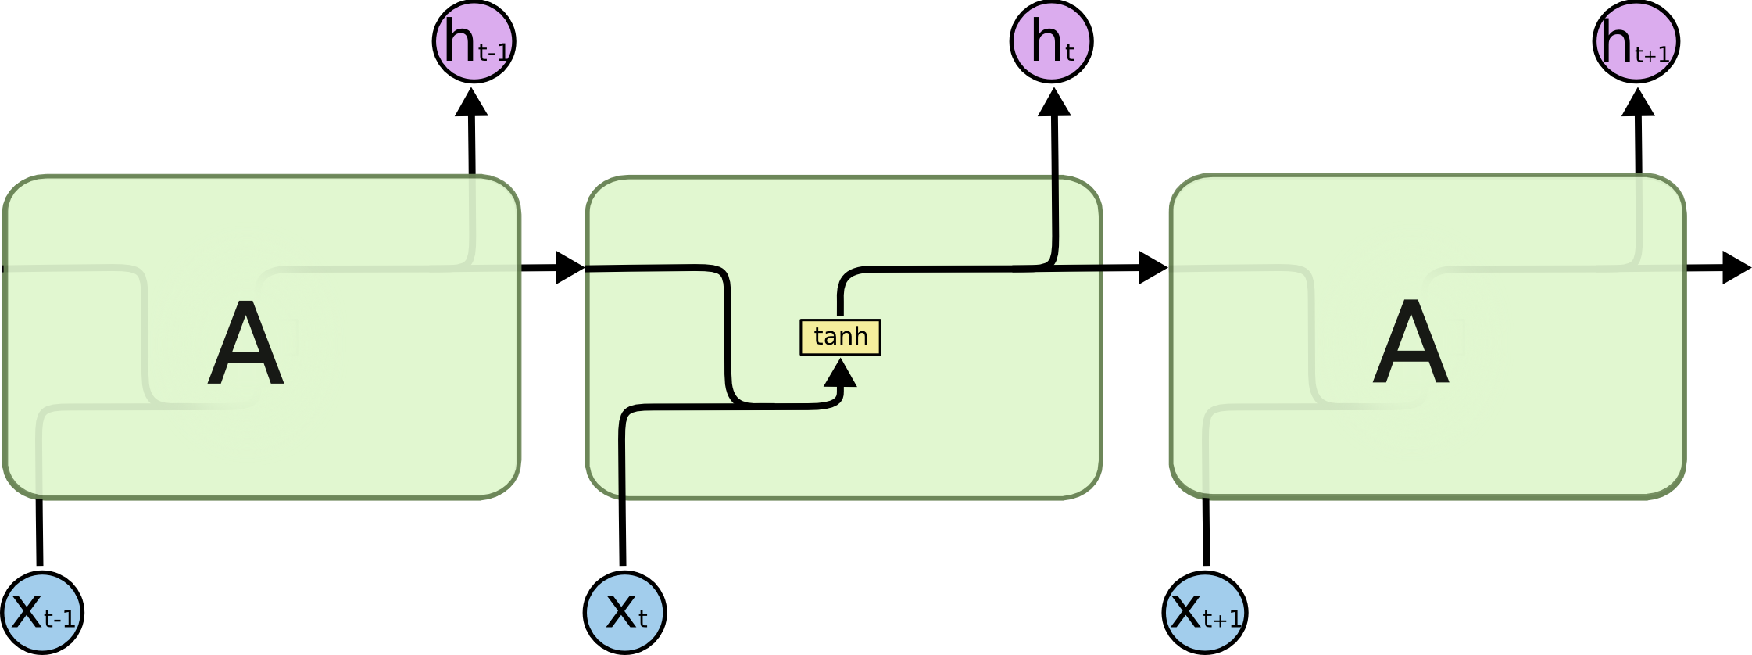
\includegraphics[width=7.3cm]{RNN.pdf}
		\end{minipage}
	}
	\subfigure[LSTM] {
		\begin{minipage}{0.48\linewidth}
			\centering
			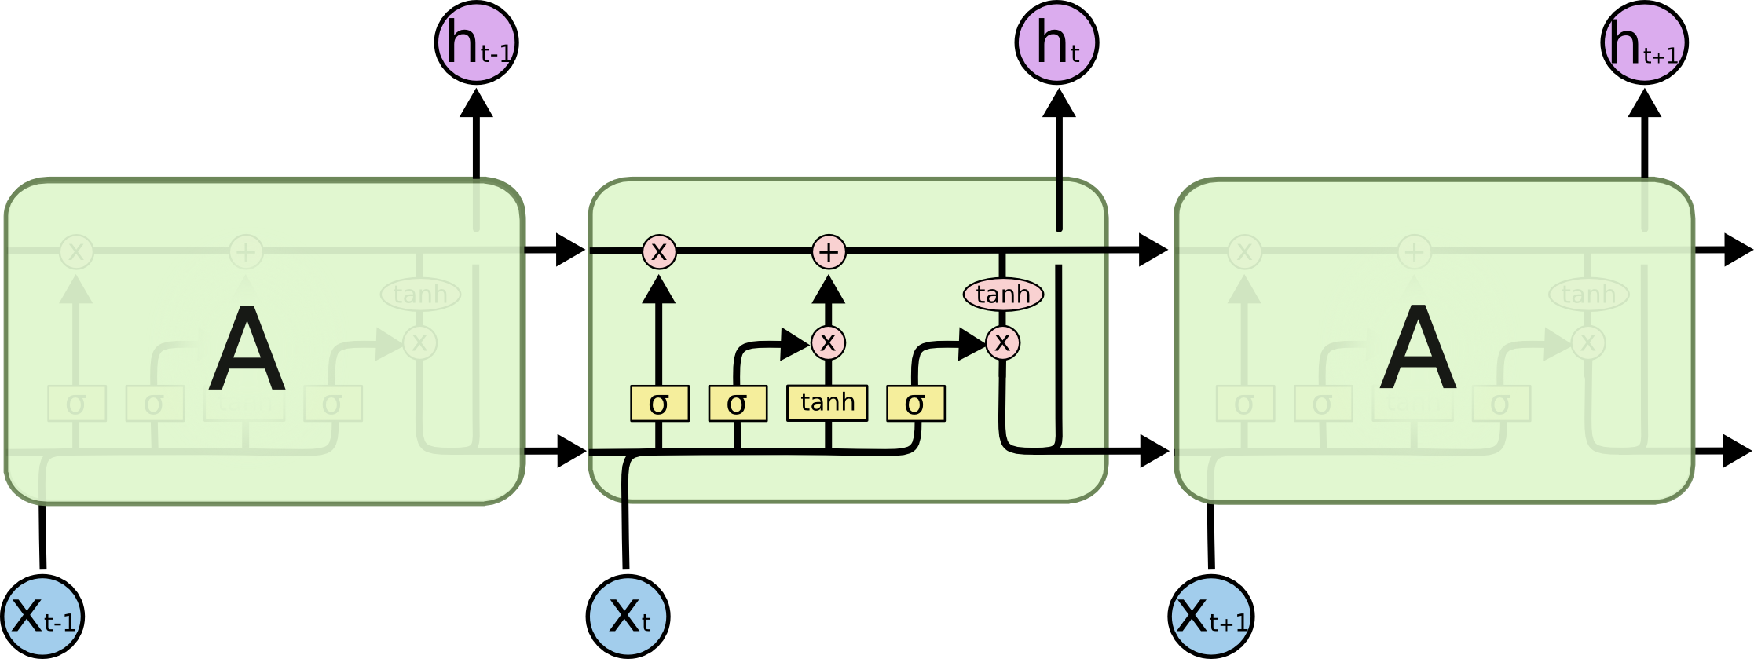
\includegraphics[width=7.3cm]{LSTM.pdf}
		\end{minipage}
	}
    \caption{RNN模型和LSTM模型的结构}
	\label{fig:structure}
\end{figure}

图\ref{fig:structure}显示了RNN模型与LSTM模型的结构,其中蓝色圆圈$x_t$表示输入信息,紫
色圆圈$h_t$表示输出信息,黄色框表示神经网络层,粉色圆圈表示逐点运算,例如矢量加法。每条
线上都承载着从一个节点的输出到另一个节点的输入的矢量。合并的线表示向量的连接,而分开的线
表示其内容被复制,然后分配到不同的位置。由图\ref{fig:structure}可见,RNN与LSTM最大的
区别在于——LSTM中最顶层多了一条信息传送带,即细胞状态$C_t$,也就是信息记忆的地方,这也是LSTM
的核心。

LSTM通过称作门(gate)的结构调节,具有删除或添加信息到细胞状态的能力。门是一种选择性地让
信息通过的方式,由$\sigma$(sigmoid)神经网络层和逐点乘法运算组成。$\sigma$层输出$0$
到$1$之间的数值,描述每个信息量可以通过多少。$0$代表“不许任何量通过”,$1$代表“允许任意
量通过”。常见的LSTM单元由一个细胞、一个输入门(input gate)、一个输出门(output gate)
和一个遗忘门(forget gate)组成。细胞会记住任意时间间隔内的值,并且三个门控制着进出单元
的信息流。

LSTM模型中,第一步是决定从细胞状态中丢弃哪些信息。这个决定通过一个称为“遗忘门层”的$\sigma$
层决定。该门会读取$h_{t-1}$和$x_t$作为输入,为细胞状态$C_t$中的每个数输出一个在$0$到$1$
之间的数值,记为$f_t$,表示保留多少信息,$1$表示“完全保留信息”,$0$表示“完全舍弃信息”。
\begin{equation}
f_t=\sigma(W_{f} \cdot [h_{t-1},x_{t}]+b_{f})
\end{equation}

第二步是在细胞状态中存储哪些信息。首先是由称为“输入门层”的$\sigma$层决定哪些信息需要更
新,该概率表示为$i_t$;然后输入门层中的tanh层创建一个新的候选值向量$\tilde{C_t}$,将其
增加到细胞状态中。
\begin{gather}
i_t=\sigma(W_{i} \cdot [h_{t-1},x_{t}]+b_i) \\
\tilde{C_t}={\rm tanh}(W_{C} \cdot [h_{t-1},x_{t}]+b_C)
\end{gather}

第三步是更新旧的细胞状态。$f_t$表示忘记上一次信息$C_t$的程度,$i_t$表示将候选值$\tilde{C_t}$
加入的程度,通过对第二步中两个信息的结合,真正实现了移除哪些旧的信息,增加哪些新信息,最
后得到了本细胞的状态$C_t$。
\begin{equation}
C_t=f_t*C_{t-1}+i_t*\tilde{C_t}
\end{equation}

最后是确定要输出的内容,即决定作出什么样的预测。首先,通过运行称为“输出门层”的$\sigma$
层来决定输出细胞状态$C_t$的哪些部分;然后,将细胞状态通过tanh层进行处理,使值在$-1$与$1$
之间,然后与$\sigma$层的输出相乘,最终输出决定输出的那部分。
\begin{gather}
o_t=\sigma(W_o \cdot [h_{t-1},x_t]+b_o) \\
h_t=o_t*{\rm tanh}(C_t)
\end{gather}

\begin{figure}[htp]
	\centering
	\subfigure[遗忘门:舍弃信息] {
		\begin{minipage}{0.48\linewidth}
			\centering
			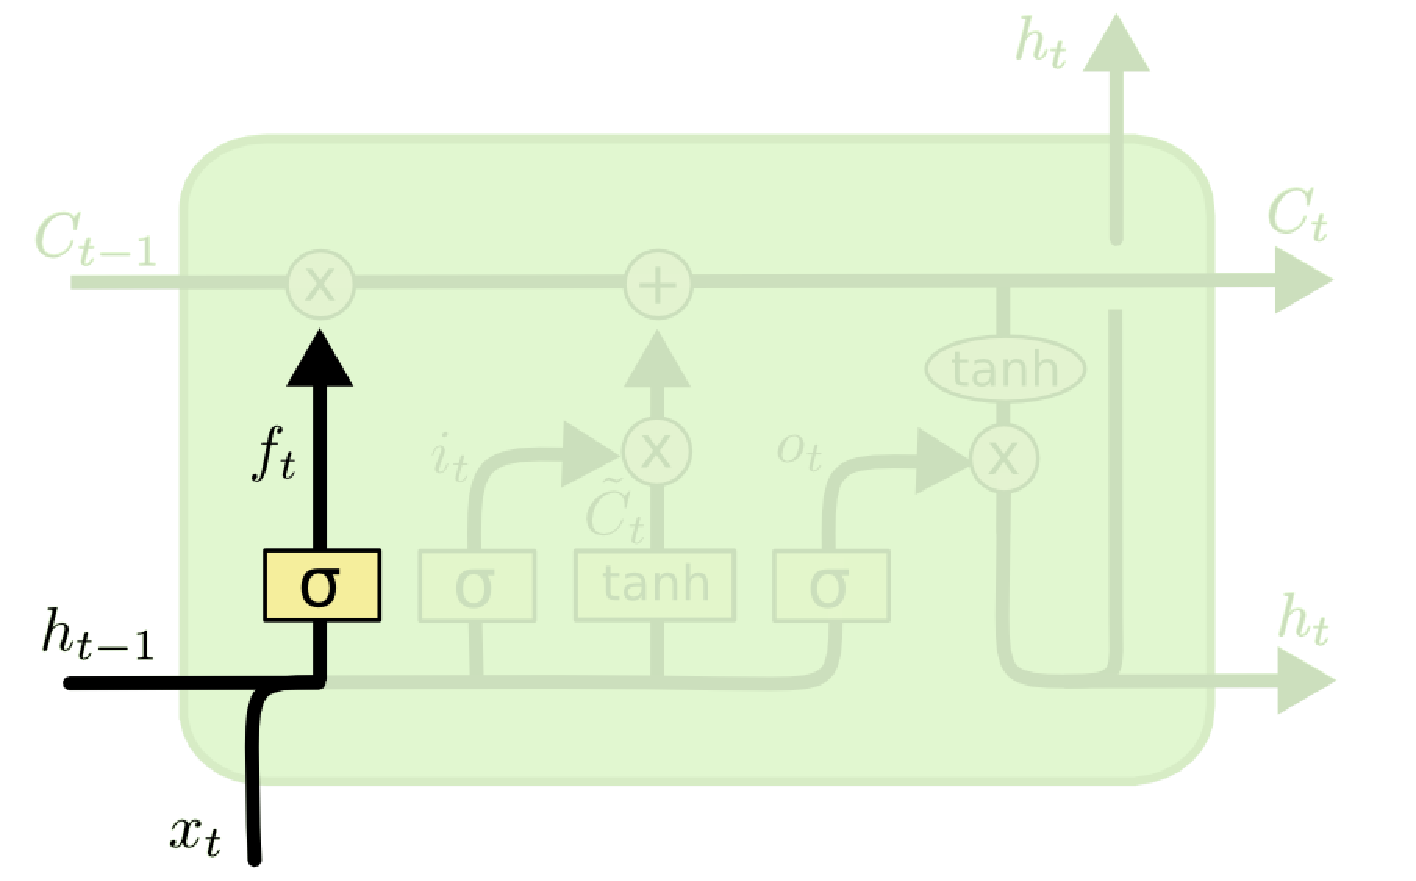
\includegraphics[width=7.0cm]{forget.pdf}
		\end{minipage}
	}
    \subfigure[输入门:存储信息] {
		\begin{minipage}{0.48\linewidth}
			\centering
			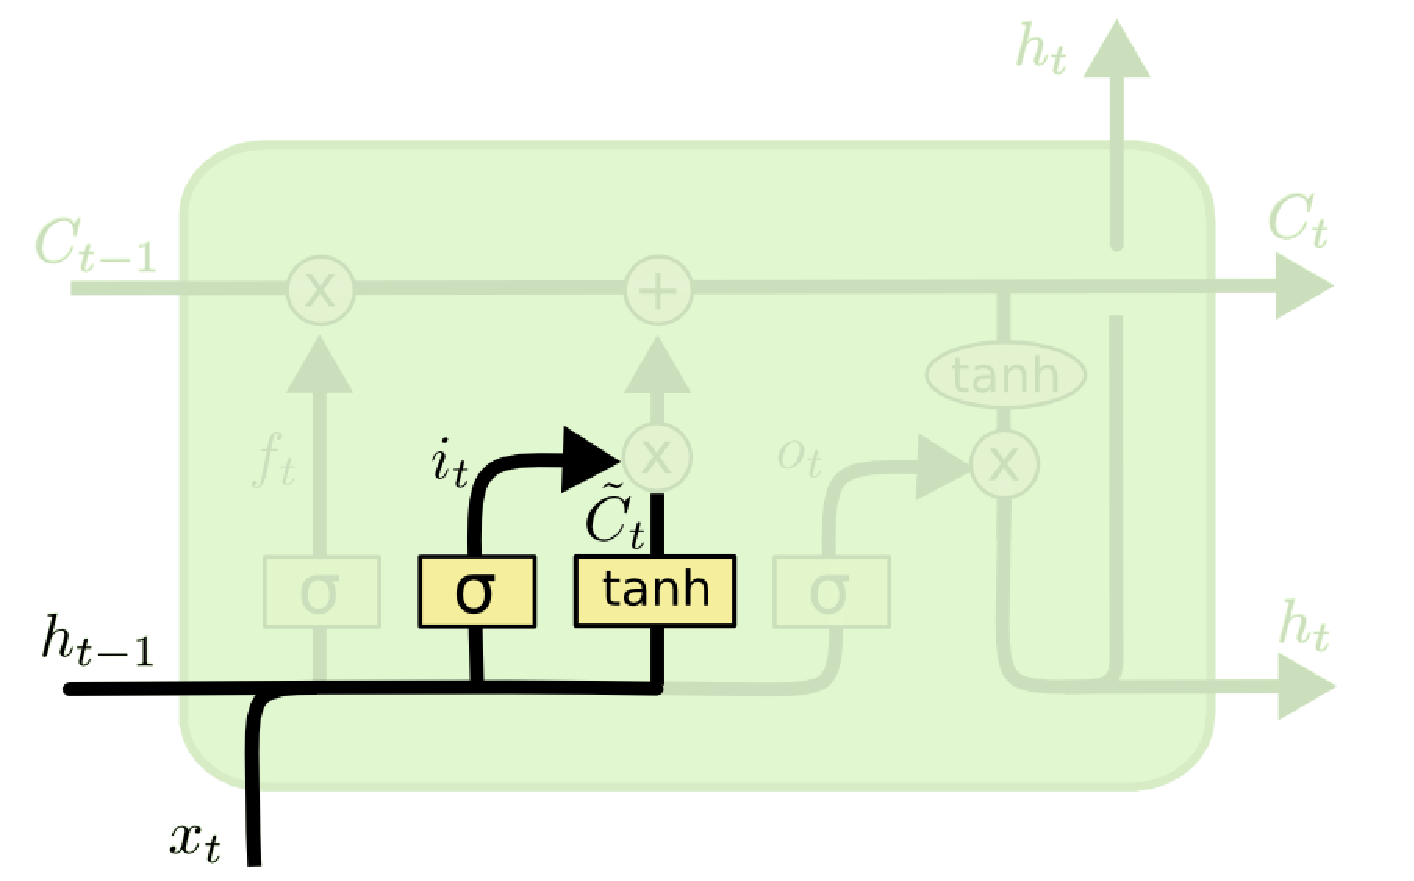
\includegraphics[width=7.0cm]{input.pdf}
		\end{minipage}
	}
	\\
	\subfigure[更新细胞状态] {
		\begin{minipage}{0.48\linewidth}
			\centering
			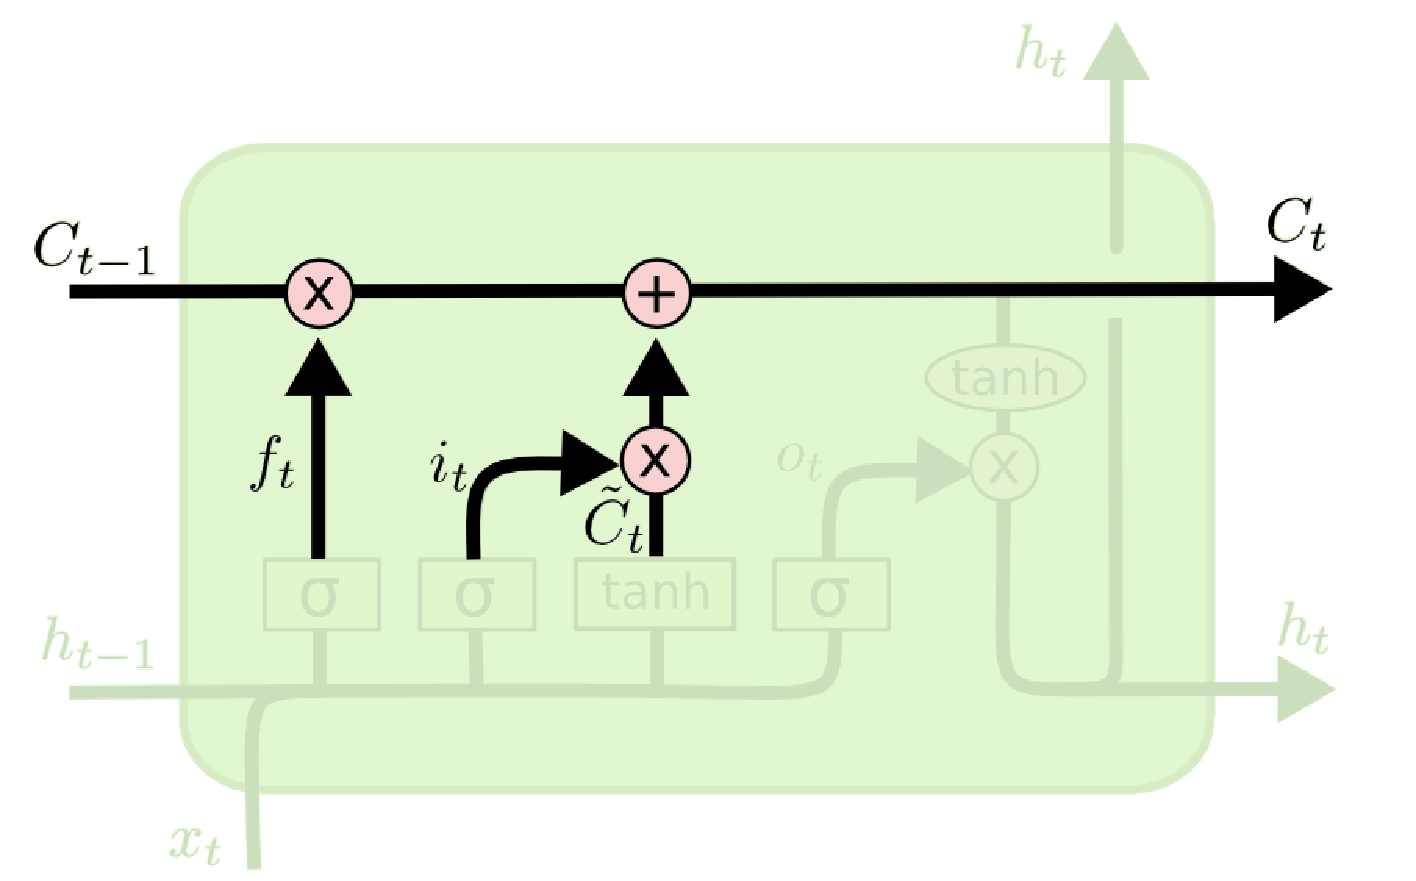
\includegraphics[width=7.0cm]{update.pdf}
		\end{minipage}
	}
	\subfigure[输出门:输出] {
		\begin{minipage}{0.48\linewidth}
			\centering
			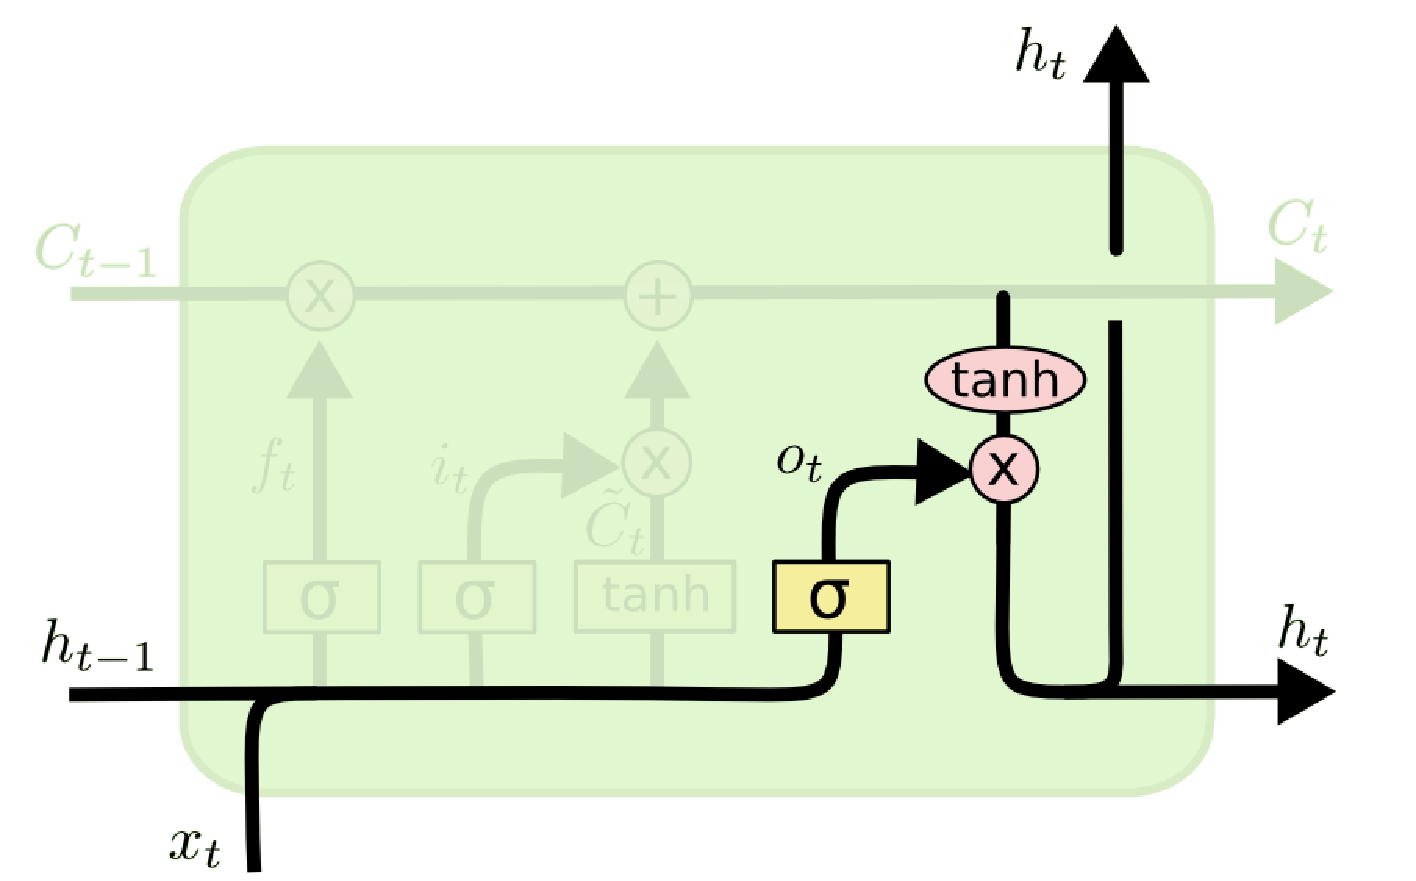
\includegraphics[width=7.0cm]{output.pdf}
		\end{minipage}
	}
    \caption{LSTM信息的流动}
	\label{fig:LSTM}
\end{figure}

\section{疫情发展现状}

本文选取了除中国外,疫情状况较为为严重的六个国家作为研究对象,分别是美国、俄罗斯、巴西、
英国、意大利、德国,以这六个国家为代表来对全球疫情数据有一个大概的分析处理。首先对六个国
家的累计确诊人数绘制折线图,以对各国疫情爆发所处阶段有一个大致了解。

从图\ref{fig:linechart}可以看出,美国确诊人数增长速度远远高于其余五个国家,在美国如此
迅猛的增势对比下,其余五国的确诊人数增长较为平缓,下面将美国从折线图中暂时去掉来对剩余的
五个国家的疫情发展现状进行展示,并将五国中最先出现第100例确诊病例的日期设定为起始日期,
即2020年2月23日。

\begin{figure}[htp]
	\centering
		\begin{minipage}{0.48\linewidth}
			\centering
			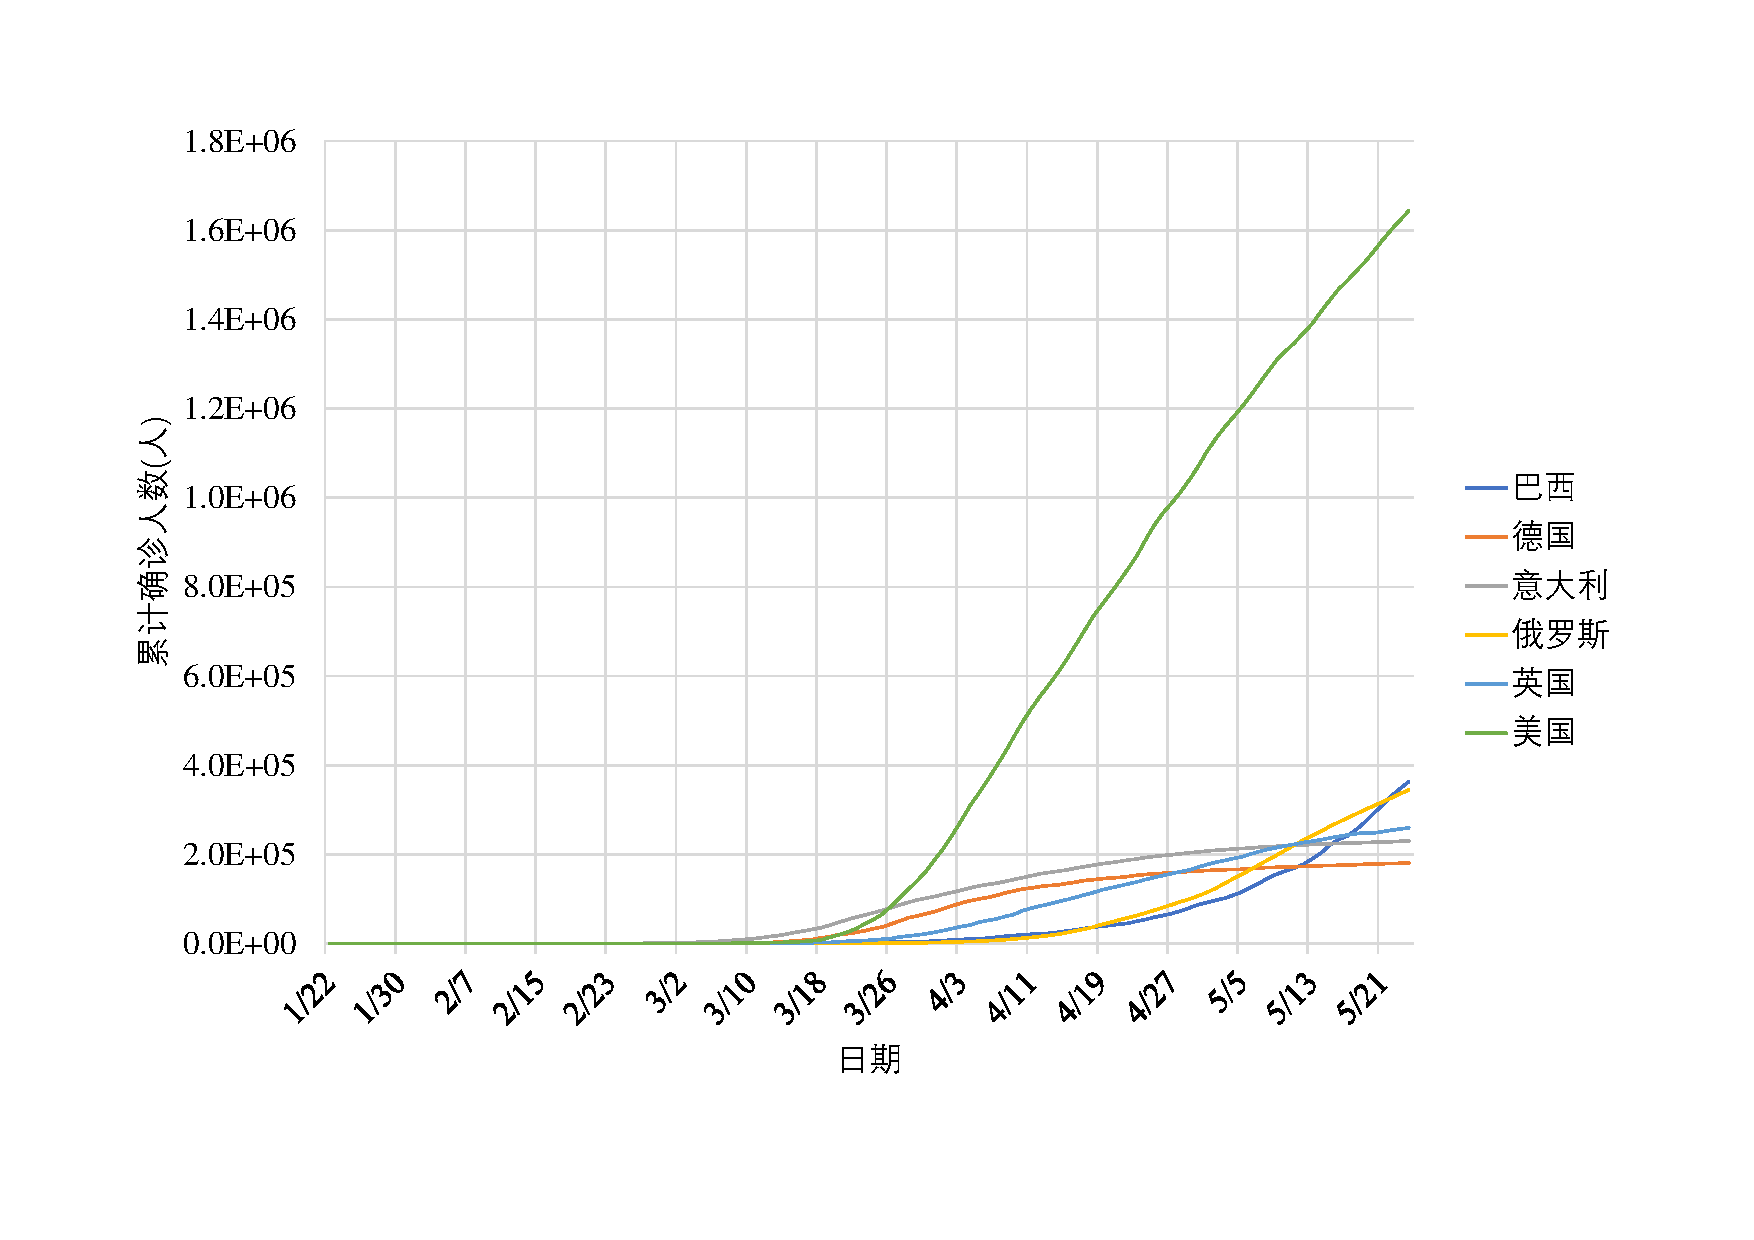
\includegraphics[width=8.8cm]{line chart.pdf}
			\caption{六个国家的累计确诊人数}
			\label{fig:linechart}
		\end{minipage}
		\begin{minipage}{0.48\linewidth}
			\centering
			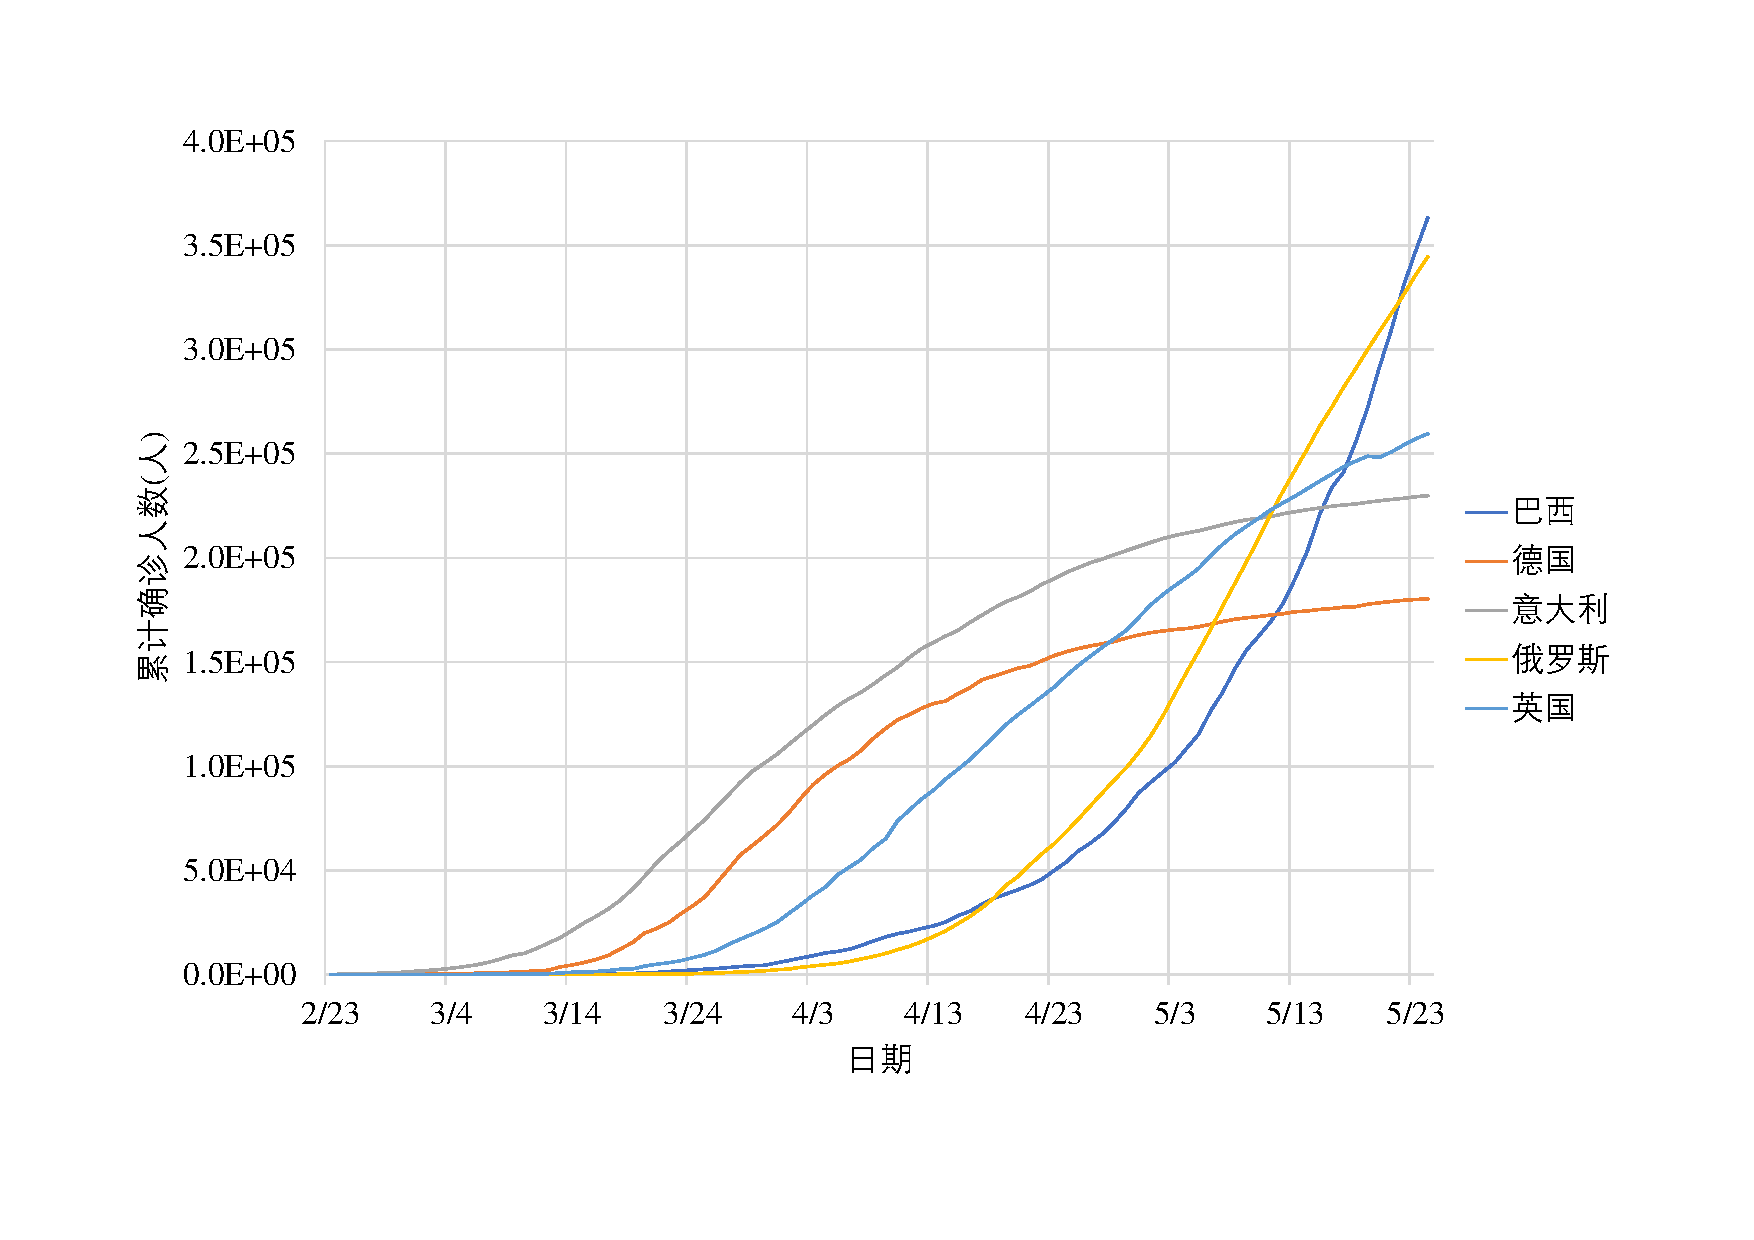
\includegraphics[width=8.8cm]{line chart without US.pdf}
			\caption{五个国家的累计确诊人数}
			\label{fig:noUS}
		\end{minipage}
\end{figure}

一般来说,疫情曲线会遵循先上升——达到顶峰——最后下降这一趋势。由图\ref{fig:noUS}可以看出,
五个国家中巴西和俄罗斯上升速度比较明显,且巴西的增长速度要明显高于俄罗斯,其余三个国家的
上升趋势依然存在,但逐渐趋于平缓,并且这五个国家的疫情均未到达其拐点及顶峰位置。由目前来
看,对疫情的防控措施不容放松,各国要坚持贯彻疫情相关管理政策及落实各种防疫措施。

\begin{table}[htp]
	\centering
	\caption{疫情数据相关指标}
	\label{index}
	\begin{tabular}{ccccc}
		\hline
		  & 累计确诊人数 & 死亡率 & 治愈率 & 占比 \\
		\hline
		巴西 & 438812	& 5.0\% & 23.6\% & 0.0022 \\
		德国 & 182452 & 2.3\%	& 42.9\% & 0.0022 \\
		意大利 & 231732& 10.4\% & 23.5\% & 0.0038 \\
		俄罗斯 & 379051 & 0.8\% & 10.4\% & 0.0026 \\
		英国 & 269127 & 11.1\% & 1.3\% & 0.0040 \\
		美国 & 1768461 & 4.5\% & 7.9\% & 0.0054 \\
		\hline
	\end{tabular}
\end{table}

进一步建立疫情数据相关指标对有助于进一步了解各国的疫情发展情况。截止5月24日,美国累计确
诊人数已经超过了176万。就累计确诊人数而言,美国不仅位居这六国之首,也是全球最多的确诊病
例国家。通过死亡率来看,俄罗斯死亡率是最低的,不足1\%,英国死亡率高达11.1\% ,是六个国
家中死亡最为严重的国家,同时,英国的治愈率也是六个国家中最低的,这个结果是由于其医疗系统
的匮乏造成的。医疗的不到位使英国对与患者的收治能力较低,病人只有在症状较为严重、较为危急
时才能得以入院治疗,对于病情严重的患者,死亡率很高和治愈率很低也就不难理解了。德国治愈率
是最高的,这跟德国工业体系的完善有很大关系,对于口罩、防护服呼吸机等这类防疫设备能做到自
主生产,最大程度地满足了德国人民的需要。而且德国在疫情爆发后,也做到了严格防控,充分隔离
。除德国外,巴西和意大利的治愈率也处在了一个相对较高的水平(23\%左右)。上表中的占比是指
该国累计确诊人数占该国总人口数的比重,可以看出美国的确诊人数占比是最多的,其次为英国。

\section{实证分析}

\subsection{数据}

本文以2020年1月22日至2020年5月24日的COVID-19疫情数据作为样本数据集。COVID-19疫情数据
来自约翰霍普金斯大学系统科学与工程中心(CSSE)提供的\href{https://github.com/CSSEGISandData/COVID-19}{COVID-19
全球数据库}。相关的各国人口数据来自\href{https://unstats.un.org}{联合国统计司}。

\subsection{SEIR模型的模拟评估}

运用SEIR模型对疫情进行预测时,本文使用了死亡率、治愈率、国家总人口,现有确诊、死亡率和治
愈率的计算公式如下:
\begin{gather}
\text{死亡率}=\frac{1}{n}\sum_{i=1}^n\frac{\text{每日累计死亡人数}}{\text{每日累计
确诊人数}} \\
\text{治愈率}=\frac{1}{n}\sum_{i=1}^n\frac{\text{每日累计治愈人数}}{\text{每日累计
确诊人数}}
\end{gather}
其中$n$为研究区间天数。

由于仍然缺乏可靠的COVID-19疫情爆发初期的数据,模型的起始日期被设定为每个国家出现第100例
确诊病例以来的日期,这表明六个受观察国家的模型起始日期不同。基于SEIR模型,本文预测了六个
国家的疫情发展趋势,六个国家的累计确诊人数的增长轨迹和预测结果如图\ref{fig:SEIRfit}和
表\ref{table:SEIRprediction}所示。

\begin{figure}[htp]
	\centering
	\subfigure[巴西] {
		\begin{minipage}{0.3\linewidth}
			\centering
			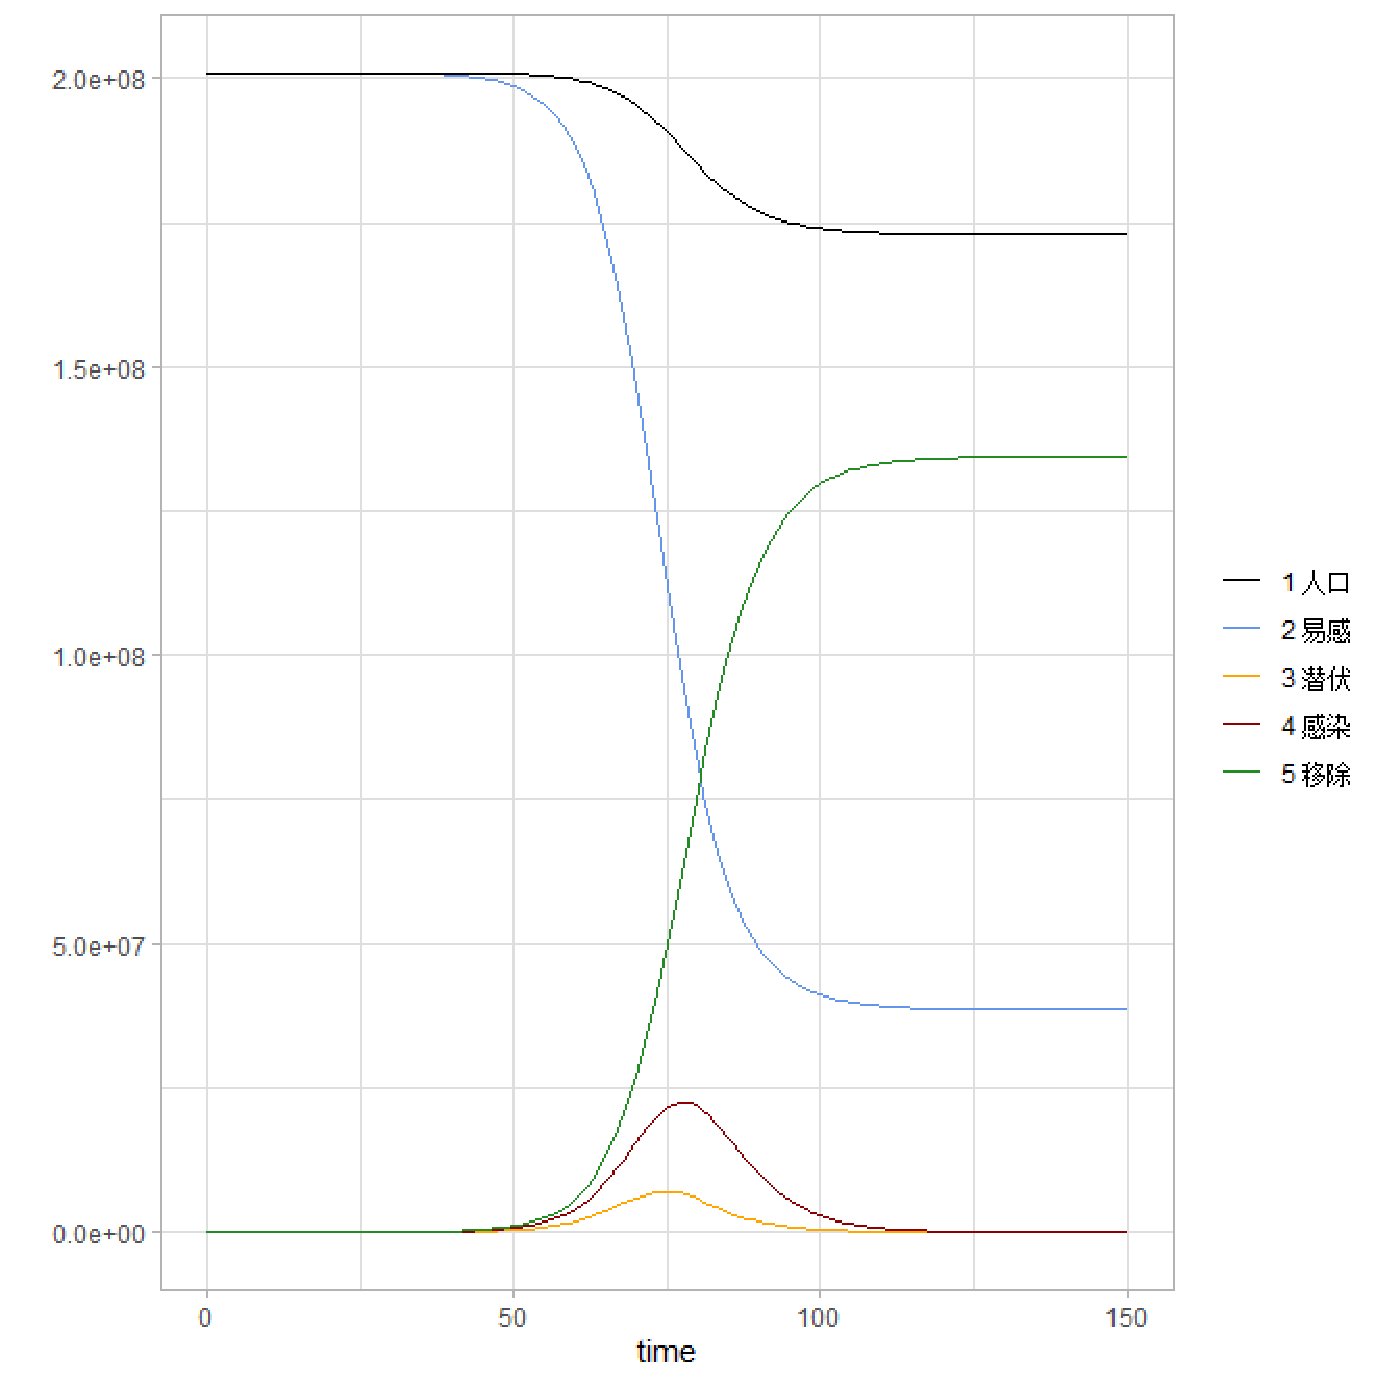
\includegraphics[width=5.0cm]{Brazil_SEIR.pdf}
		\end{minipage}
	}
	\subfigure[德国] {
		\begin{minipage}{0.3\linewidth}
			\centering
			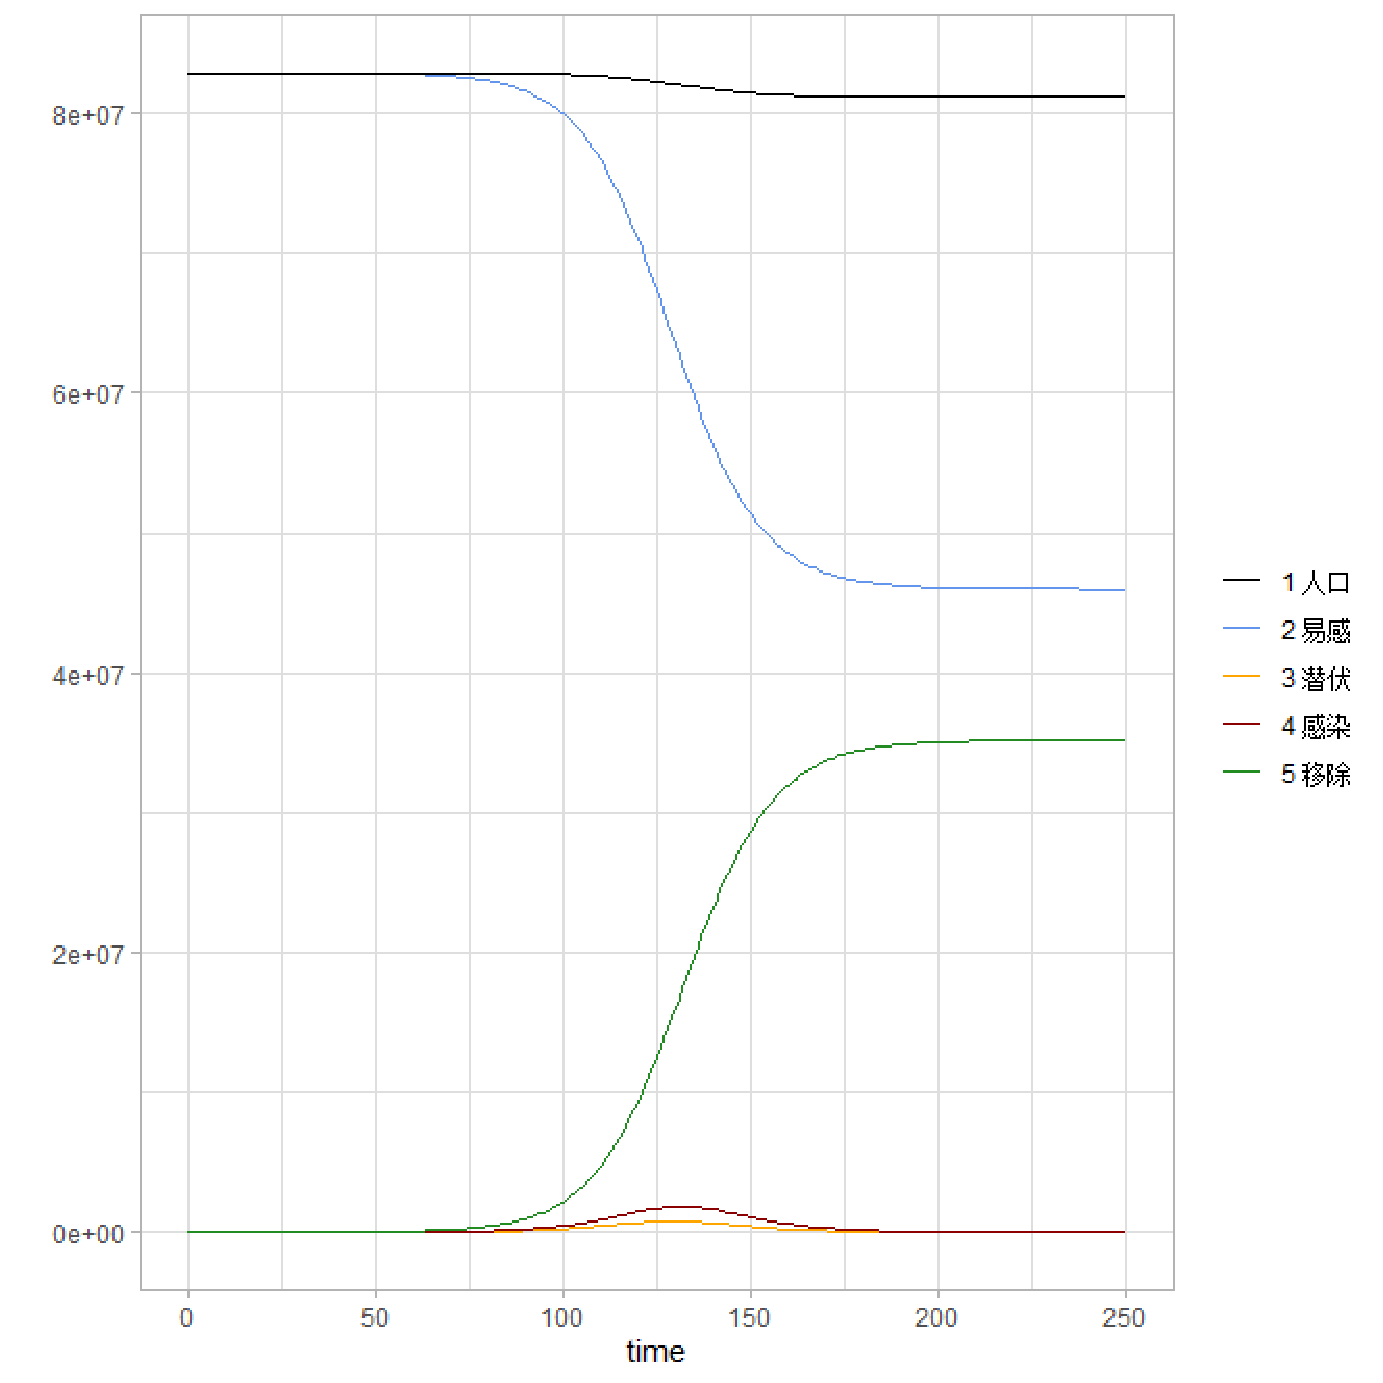
\includegraphics[width=5.0cm]{Germany_SEIR.pdf}
		\end{minipage}
	}
	\subfigure[意大利] {
		\begin{minipage}{0.3\linewidth}
			\centering
			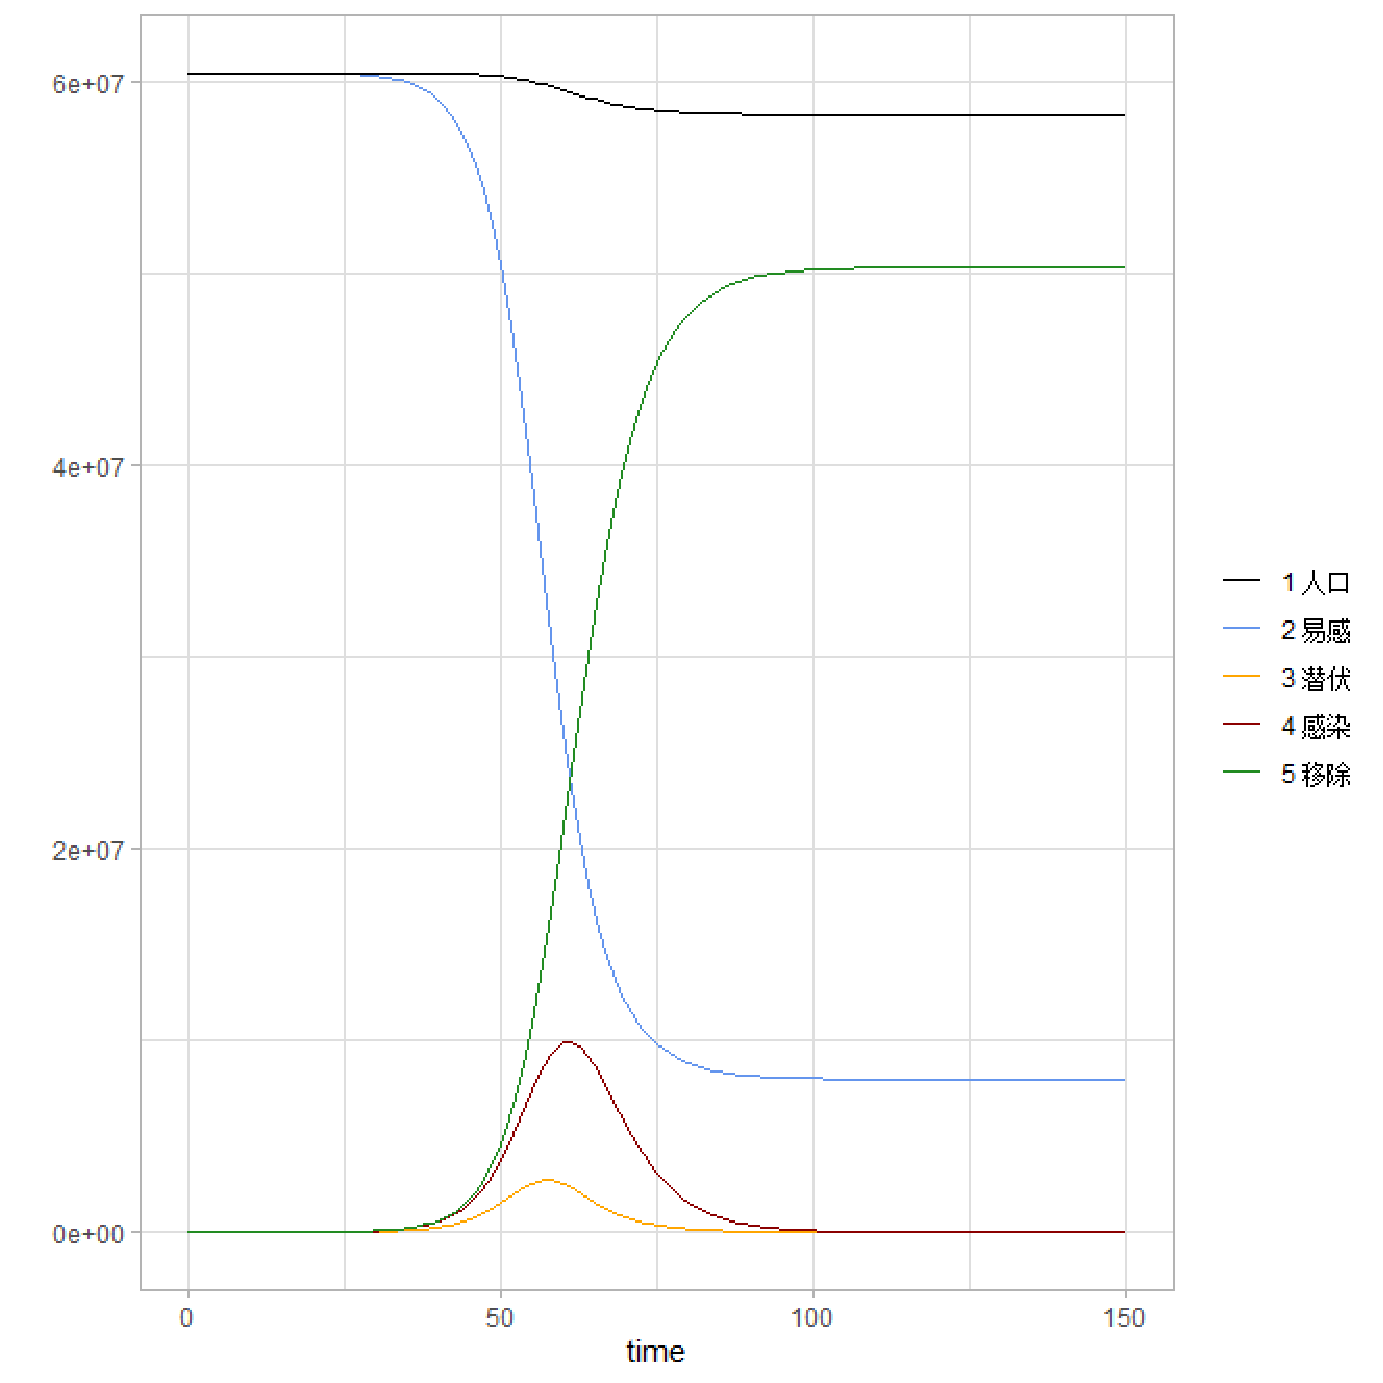
\includegraphics[width=5.0cm]{Italy_SEIR.pdf}
		\end{minipage}
	}
    \\
	\subfigure[俄罗斯] {
		\begin{minipage}{0.3\linewidth}
			\centering
			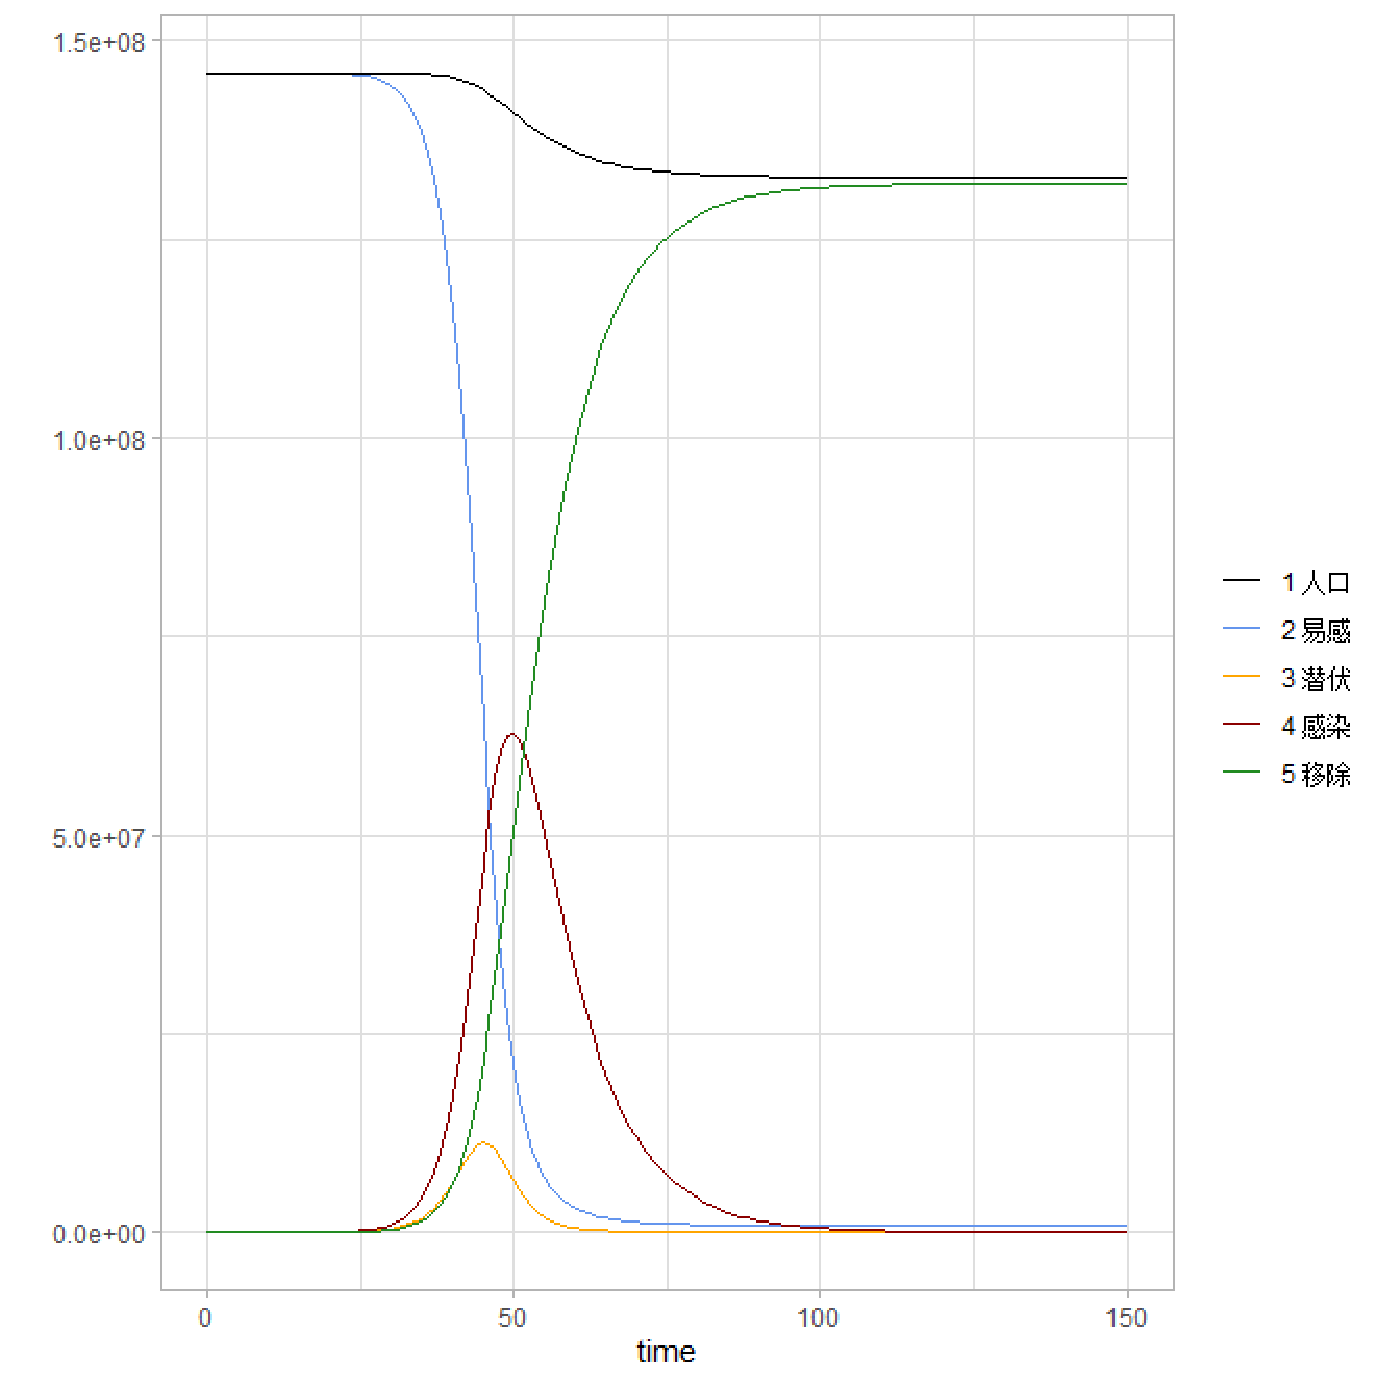
\includegraphics[width=5.0cm]{Russia_SEIR.pdf}
		\end{minipage}
	}
    \subfigure[英国] {
    	\begin{minipage}{0.3\linewidth}
    		\centering
    		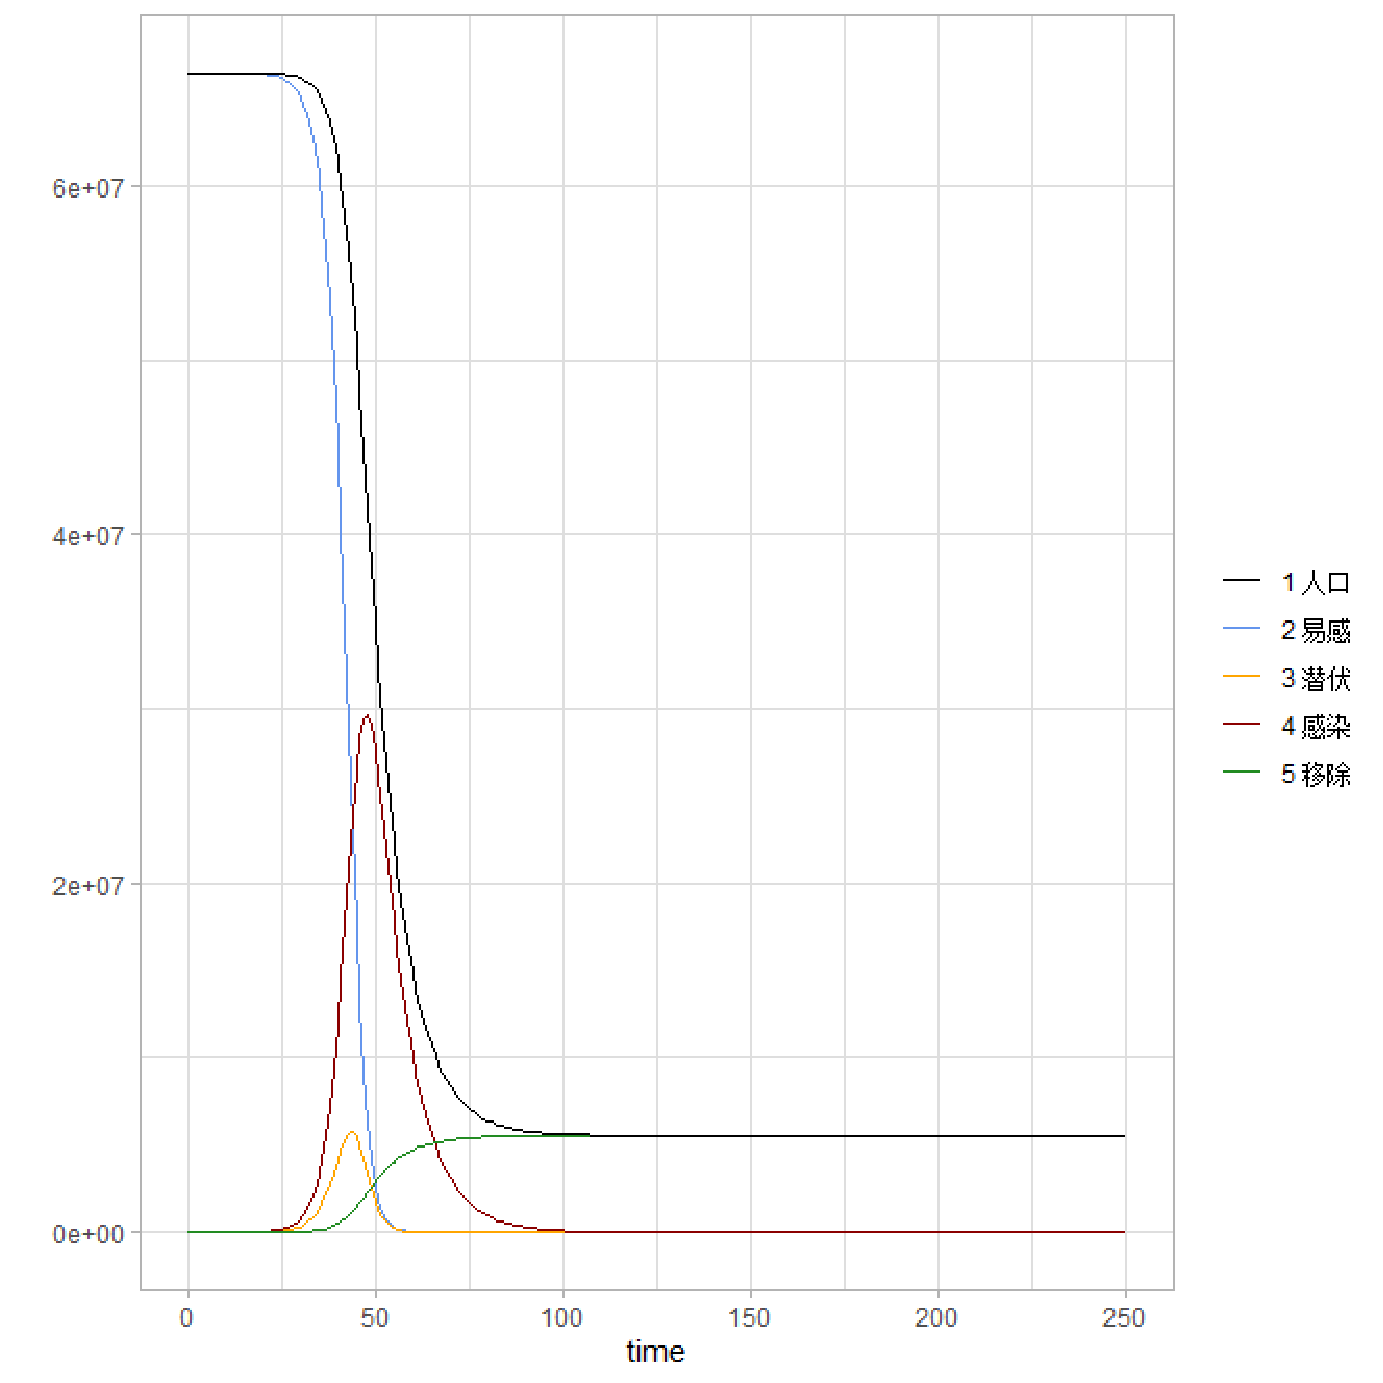
\includegraphics[width=5.0cm]{UK_SEIR.pdf}
    	\end{minipage}
    }
    \subfigure[美国] {
    	\begin{minipage}{0.3\linewidth}
    		\centering
    		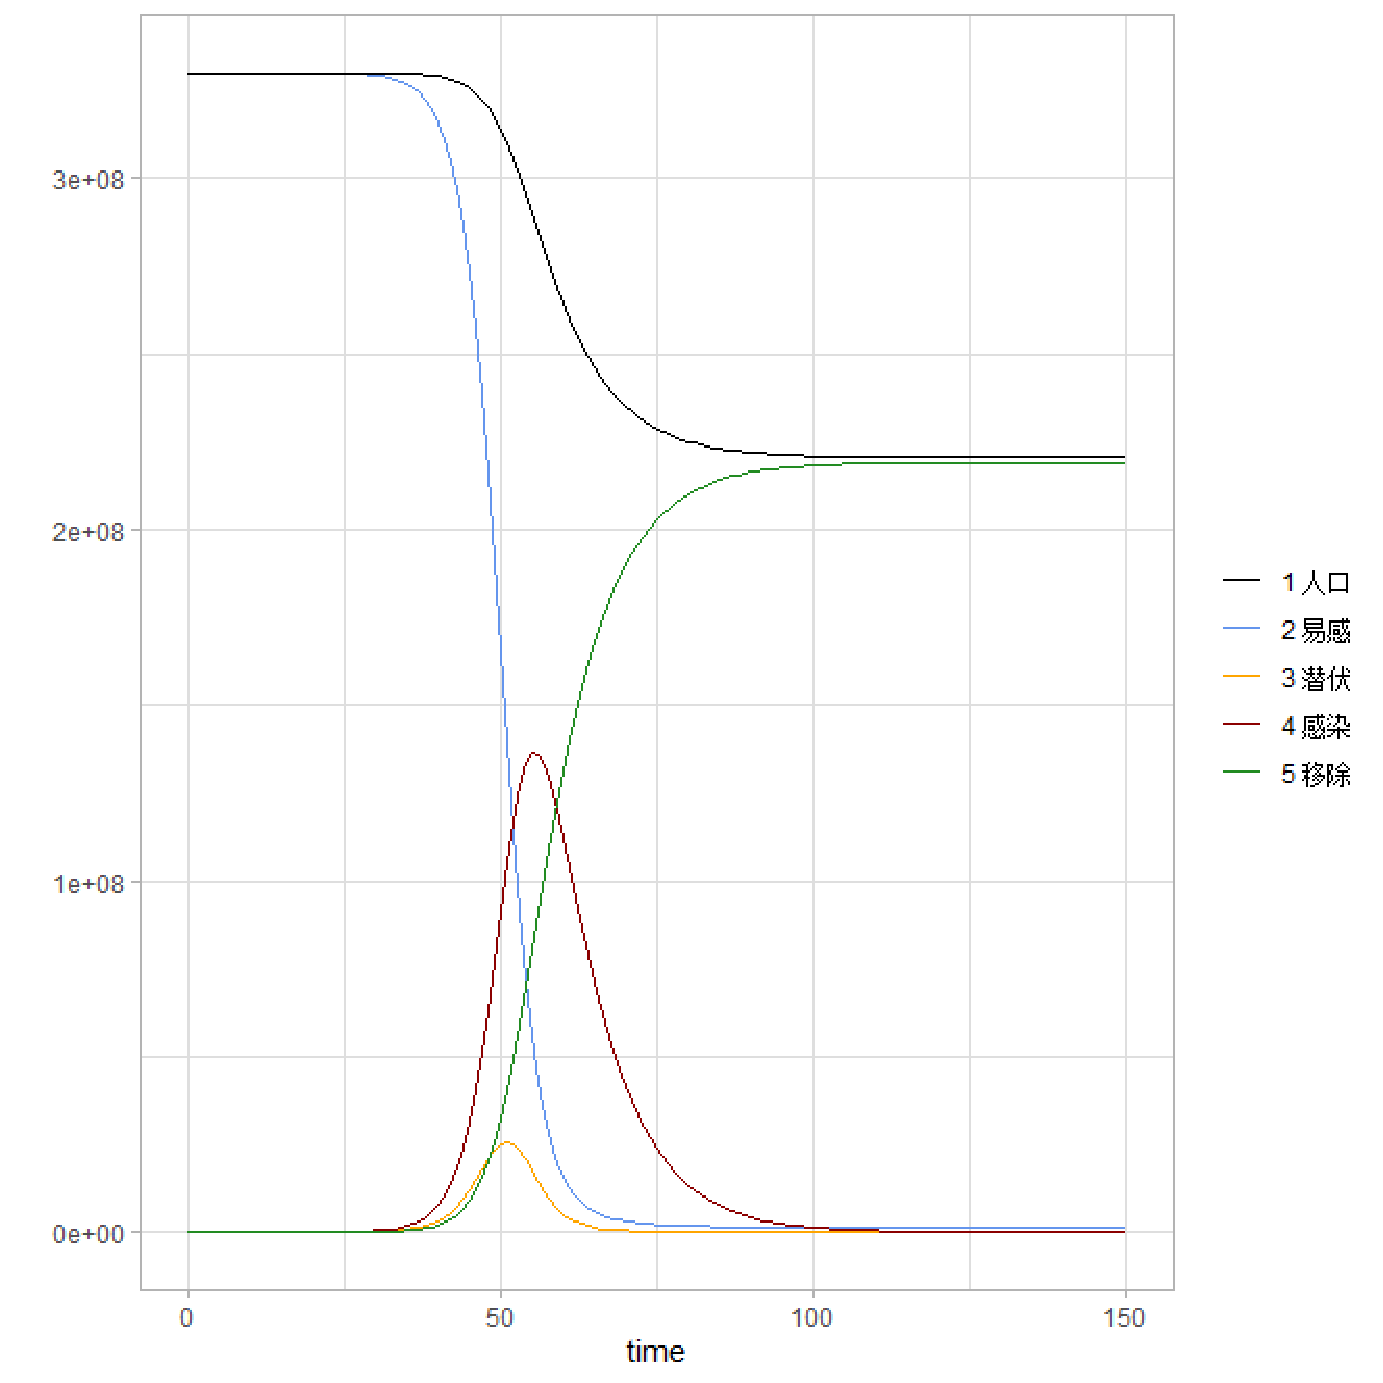
\includegraphics[width=5.0cm]{US_SEIR.pdf}
    	\end{minipage}
    }
	\caption{SEIR模型的模拟}
	\label{fig:SEIRfit}
\end{figure}

\begin{table}[htp]
	\centering
	\caption{六个国家的疫情高峰预测}
	\label{table:SEIRprediction}
	\begin{tabular}{cccccccc}
		\hline
		 & 巴西 & 德国 & 意大利 & 俄罗斯 & 英国 & 美国 \\
		\hline
		高峰日 & 81 & 169 & 85 & 51 & 49 & 55 \\
		峰值(*$10^4$) & 2261.3 & 104.3 & 499.5 & 6290 & 2965.8 & 13643 \\
		\hline
	\end{tabular}
\end{table}

从图\ref{fig:SEIRfit}中可以看出,在疫情发生后,英国的易感人数会有一个大幅下降,即潜伏
期人数的增加幅度比较大,感染人数和易感人数交叉时感染人数会达到顶峰。模型预测,法国会在初
始日期49天后达到这个顶峰,也就是月日累计确诊人数达到顶峰,预测峰值为2965.8万人。相较于
法国,德国易感人数下降的幅度较少,感染人数和易感人数并未有交叉,模型预测德国在169天累计
确诊人数达到峰值,时间跨度较长。总体上看,德国疫情扩散相对比较稳定,且预测峰值人数也是六
个国家中最少的,预测峰值人数为104.3万人。不同于别的国家,英国的SEIR曲线,易感人数和全国
总人口在预测期间急速下降,最终停在了一个较低的水平,表明英国的疫情扩散极其迅速以及蔓延的
后果(参照其死亡率及治愈率)特别严重。截至目前,英国累计确诊人数增长还是处在一个上升的状态,
如果英国政府不采取更加严格的措施,模型预测结果很有可能成为现实。模型预测英国的峰值日期来
临时间很短,将其设定在了初始日期后的49天,并预测最终累计确诊人数会超过2900万人,这个预
测结果应该得到政府的重视。从美国的SEIR模型图中可以看出美国峰值感染人数处在一个极高的水平,
在模型达到稳定后,国家总人口与移出人数十分接近,这表明,照目前美国传播速度,在疫情发展后
期,美国大部分公民都将感染新型冠状病毒,易感人数数量极低,模型将峰值日期设定在了初始日期
后的55天,并预测最终累计确诊人数会超过13000万人,为六个国家中预测的累计确诊人数之最。由
于俄罗斯治愈率相对较低,在疫情发生后的第25—35天,潜伏状态和感染状态的人数开始加速增长,
在第41—51天达到高峰,随后开始下降。模型预测俄罗斯的感染人数峰值在500万以上,相对较高。
并且,在疫情结束后,俄罗斯累计确诊人数占全国总人数的比例也相对较高。意大利的SEIR模型仿真
结果,可以看出在疫情发展初期,潜伏状态和感染状态的人数在都处于上升趋势,在第30天—40天左
右开始加速增长,在第75天—85天达到高峰,之后开始下降直至消失。而在疫情结束后累计确诊人数
达到499万人。巴西与意大利的SEIR结果较为相似,但不同的是,模型将巴西的峰值日期设立在了起
始日期后的70—81天,较意大利峰值来临较早一点,但峰值累计确诊人数却远大于意大利,模型预测
峰值达2261.3万人,疫情扩张的结果也相当严重。

\subsection{LSTM模型的模拟评估}

对于LSTM时间序列中的每个细胞状态,该单元从4个连续的日期中获取病例计数,并输出随后的第5
个日期的预测。本文的LSTM模型是使用{\em Keras}训练的。应用以下五种优化算法:{\em Adam}
、{\em SGD}、{\em AdaDelta}、{\em Adagrad}和{\em 
RMSProp},并结合以下四种损失函数:{\em MSE}、{\em MAE}、{\em Huber}以及{\em Log 
Cosh},比较了上述20种组合在最小化损失方面的性能。

\begin{figure}[htp]
	\centering
	\subfigure[MSE] {
		\begin{minipage}{0.48\linewidth}
			\centering
			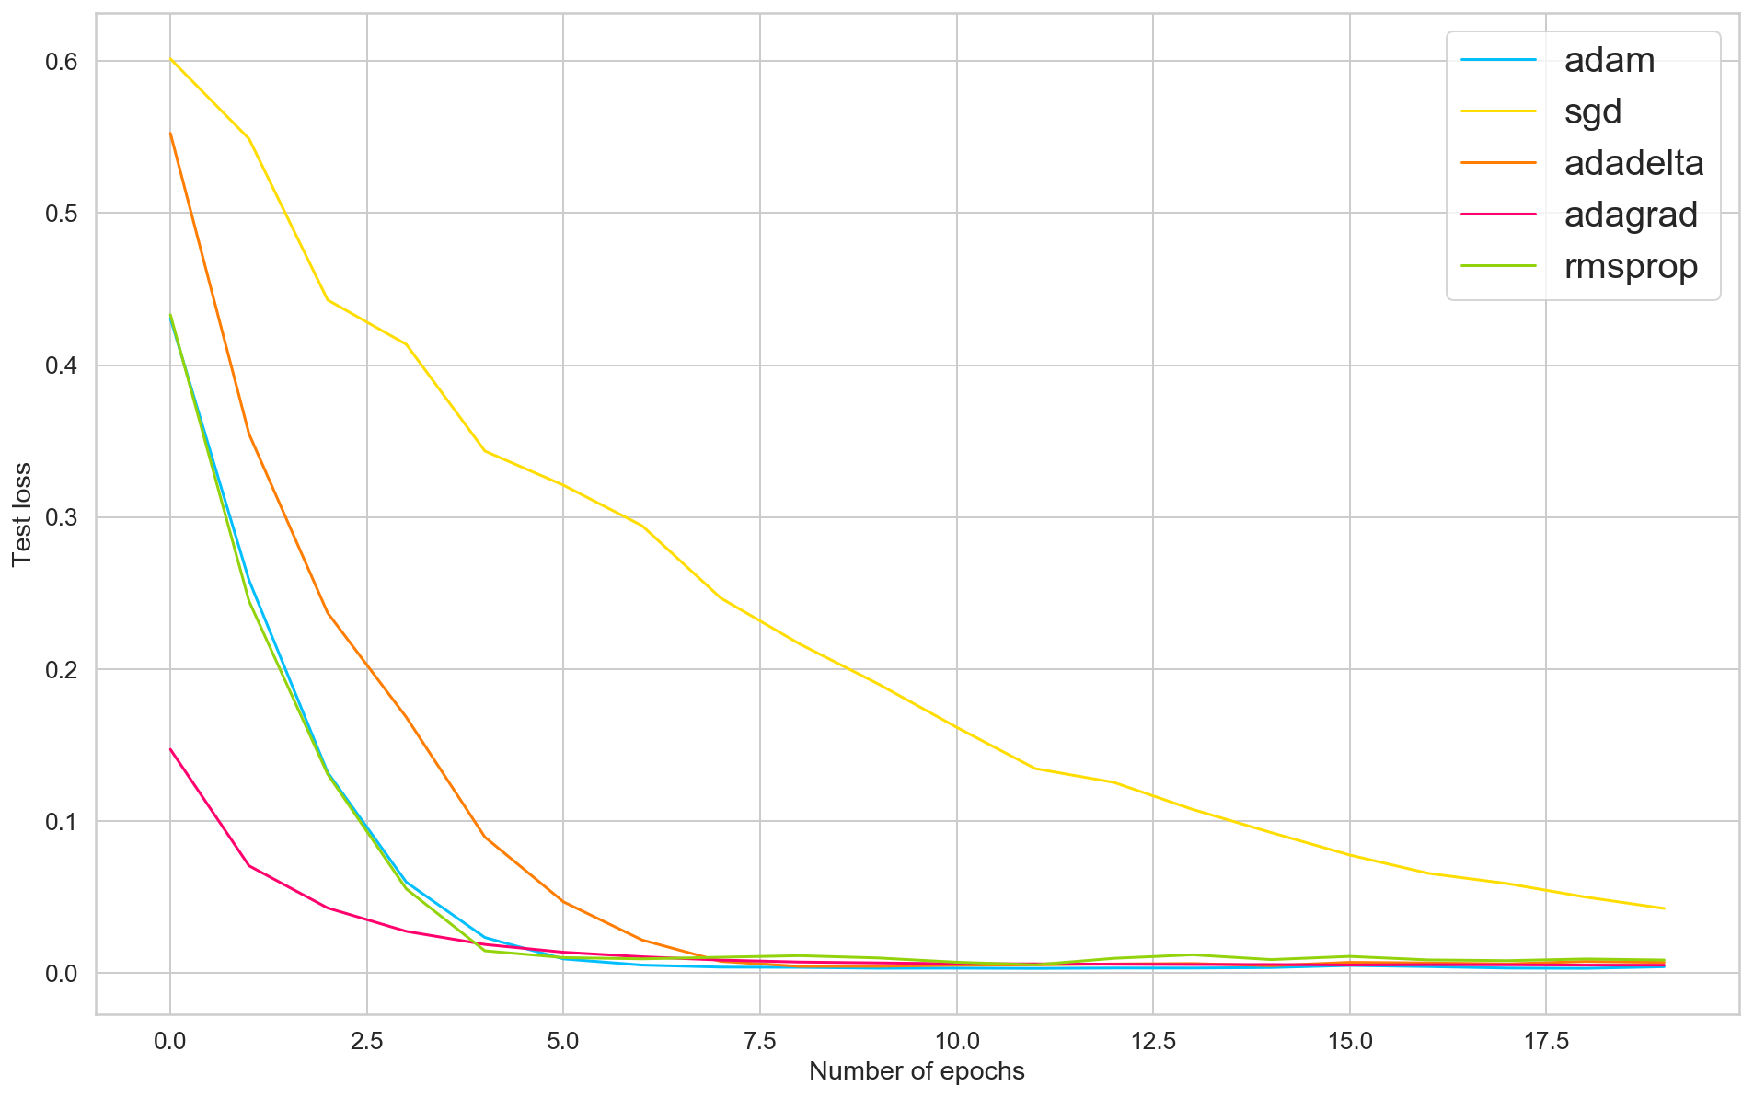
\includegraphics[width=7.0cm]{MSE.pdf}
		\end{minipage}
	}
	\subfigure[MAE] {
		\begin{minipage}{0.48\linewidth}
			\centering
			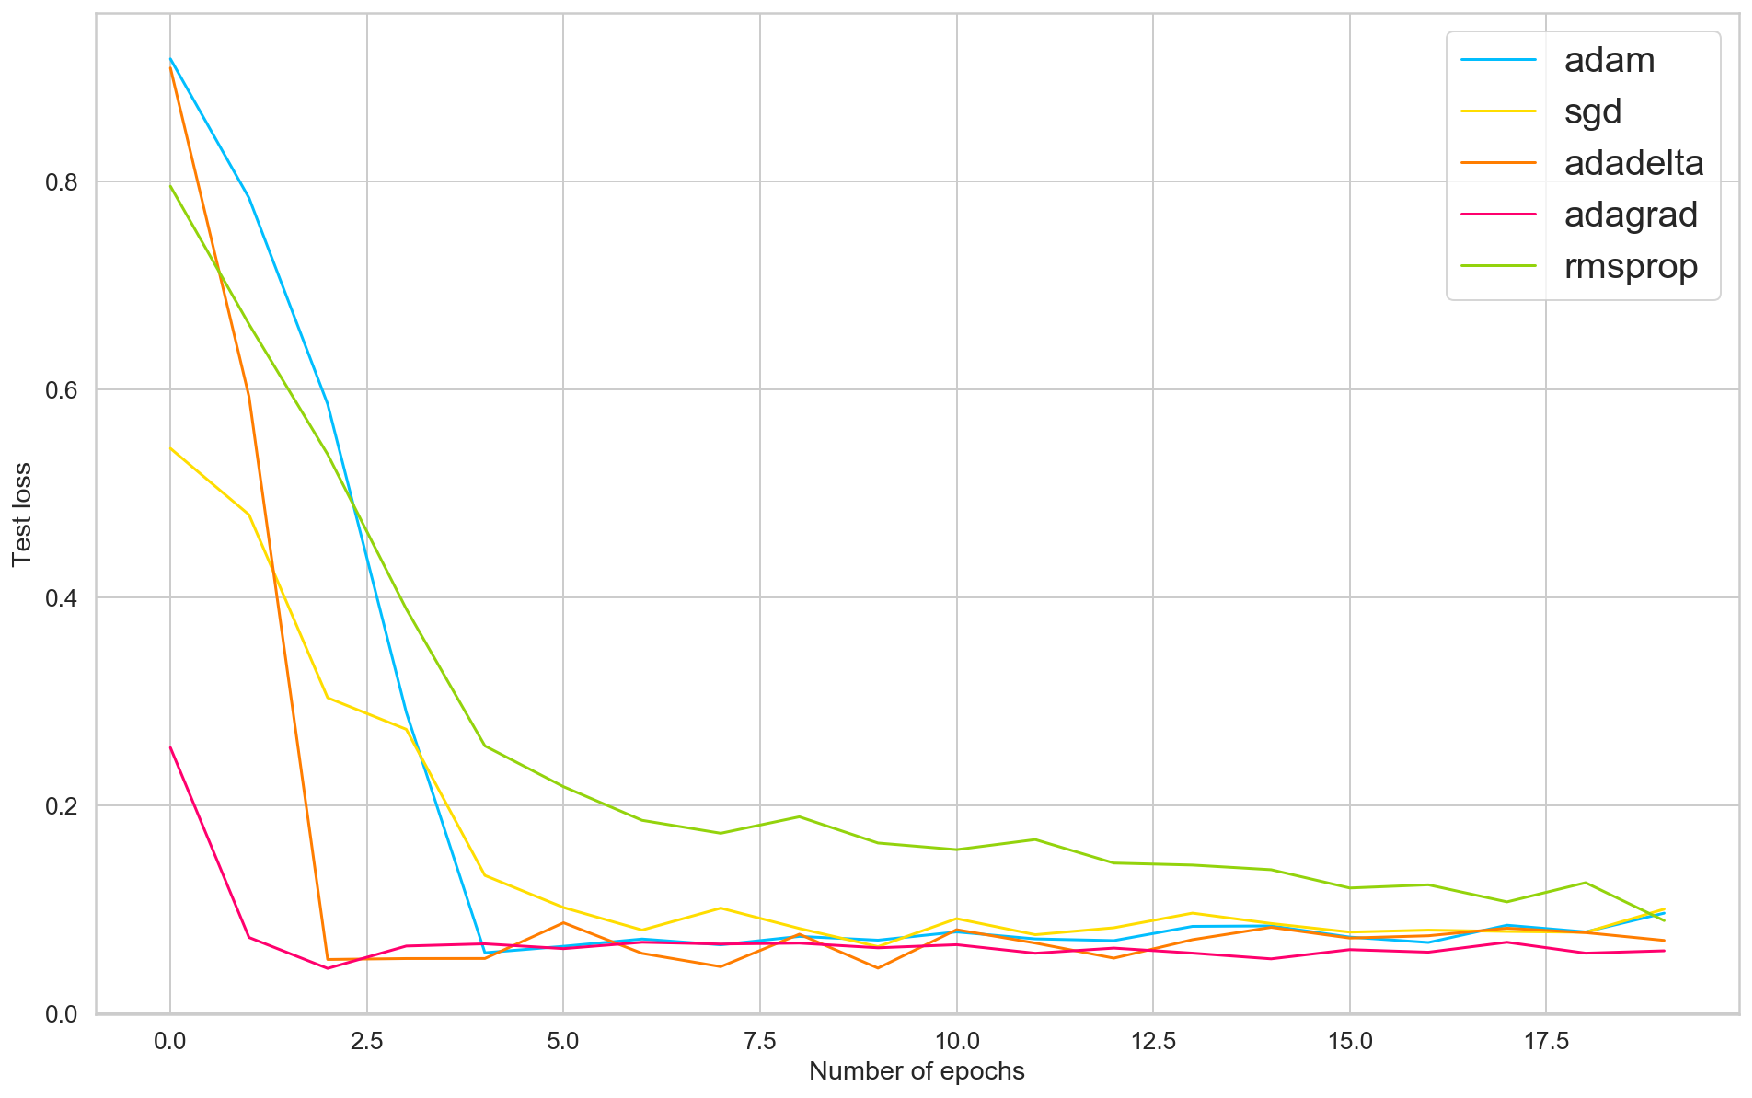
\includegraphics[width=7.0cm]{MAE.pdf}
		\end{minipage}
	}
	\\
	\subfigure[Huber] {
		\begin{minipage}{0.48\linewidth}
			\centering
			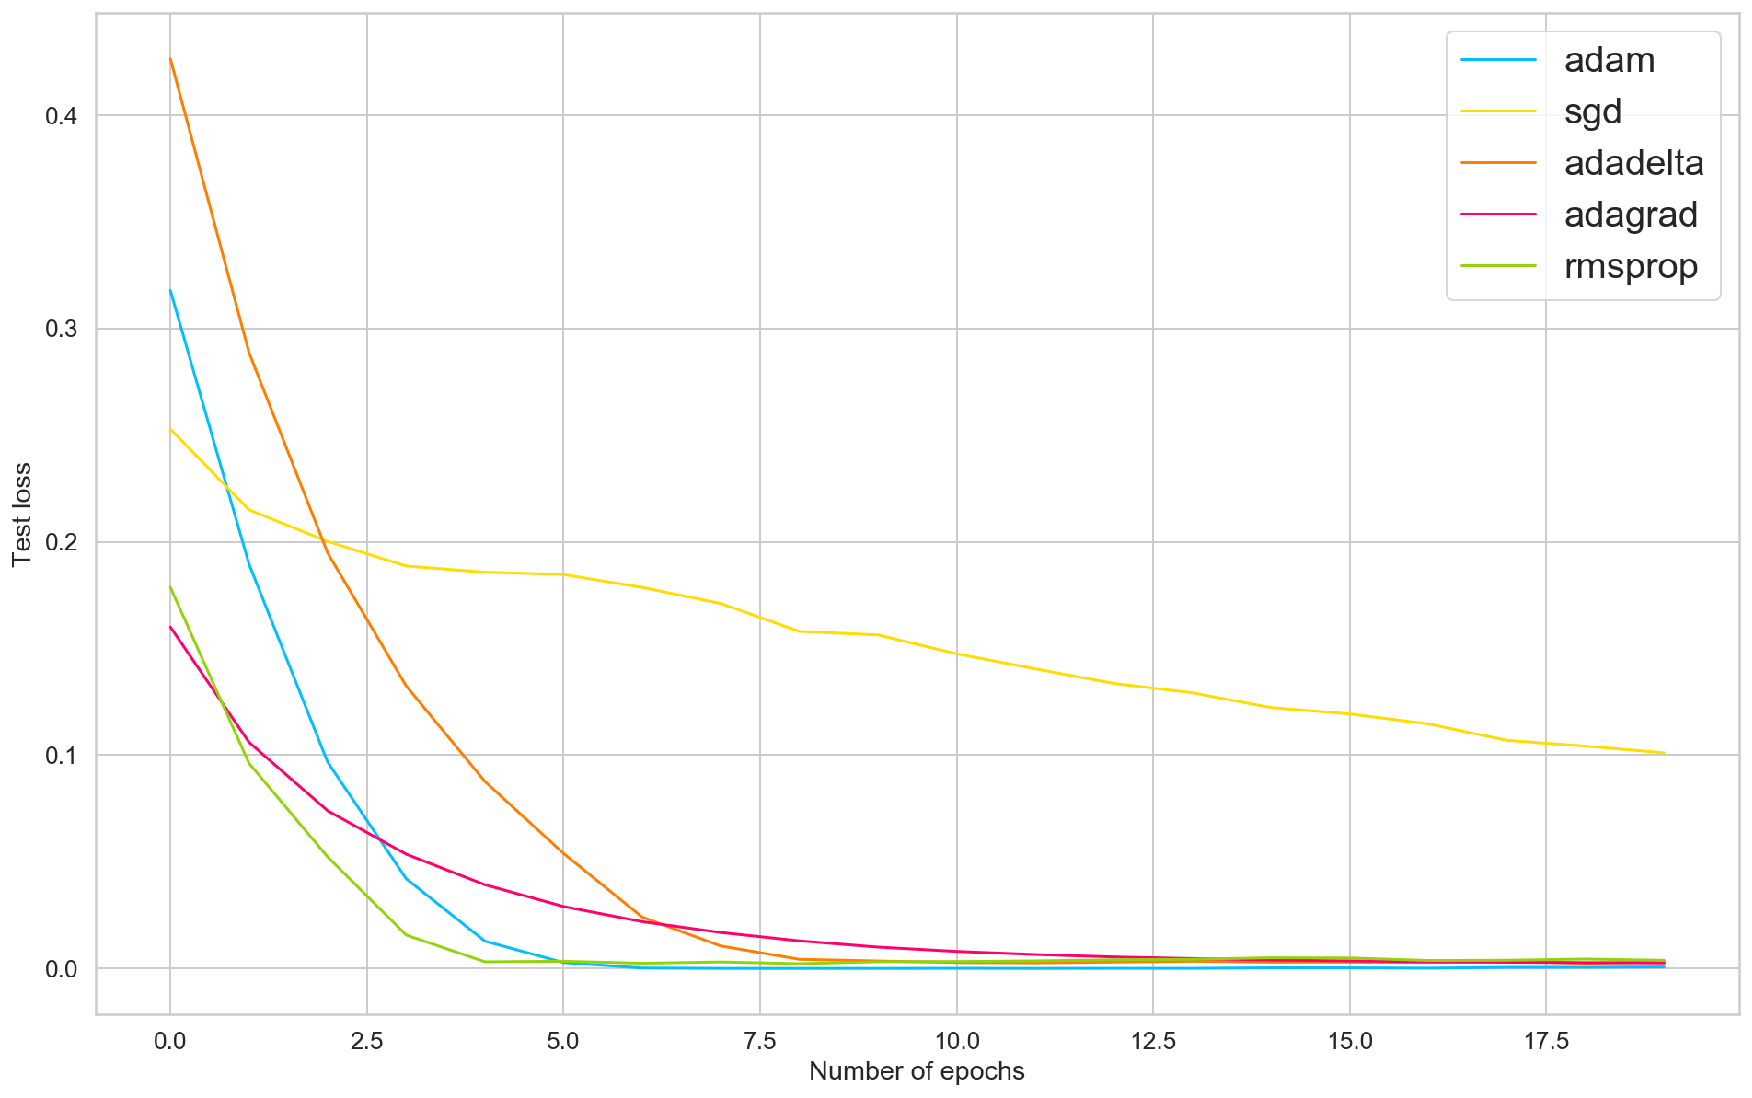
\includegraphics[width=7.0cm]{Huber.pdf}
		\end{minipage}
	}
	\subfigure[Log Cosh] {
		\begin{minipage}{0.48\linewidth}
			\centering
			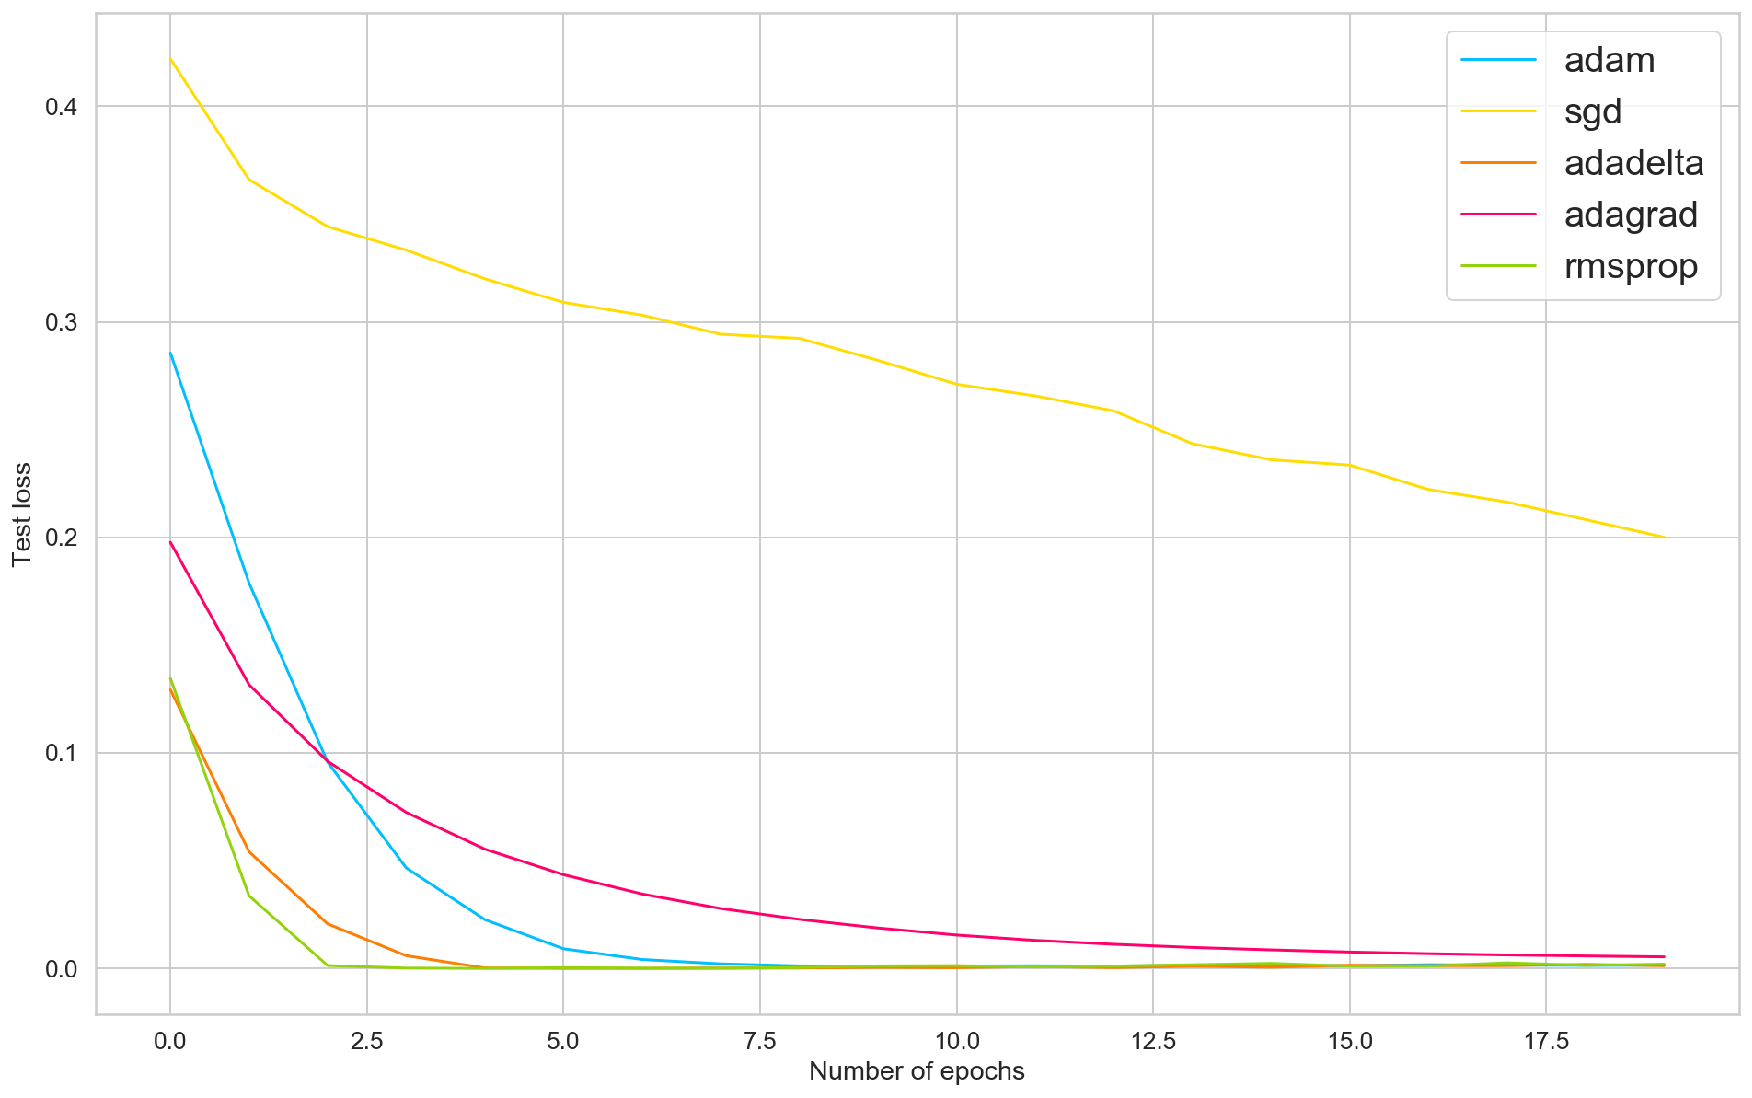
\includegraphics[width=7.0cm]{LogCosh.pdf}
		\end{minipage}
	}
	\caption{不同损失函数和优化器之间的性能比较}
	\label{fig:optnloss}
\end{figure}

如图\ref{fig:optnloss}所示,SGD是性能最差的优化器,其原因可能是SGD无法适应学习率,没有
设置动量,训练不稳定,导致它总是围绕局部的极小值反弹波动。MAE是最差的损失函数,每个优化
器都没有收敛到接近于零。尽管AdaDelta、AdaGrad和RMSProp在某些特定情况下的性能良好,但本
文在接下来的实证中选择了Adam优化器和MSE损失函数相结合,因为它的收敛速度性能较为一致。并
且,通过比较了模型在不同训练轮数(epoch)和预测步长(lookback)时的表现,最终选用训练轮数
为70、预测步长为4。这可能是因为模型运行过少或过多会导致训练不足或训练过度,使得数据的拟
合不足或过度拟合。将最末7天的数据集作为测试集,其余作为测试集,对各个国家的数据进行训练,
LSTM训练模拟结果如图\ref{fig:LSTMfit}所示。

\begin{figure}[htp]
	\centering
	\subfigure[巴西] {
		\begin{minipage}{0.3\linewidth}
			\centering
			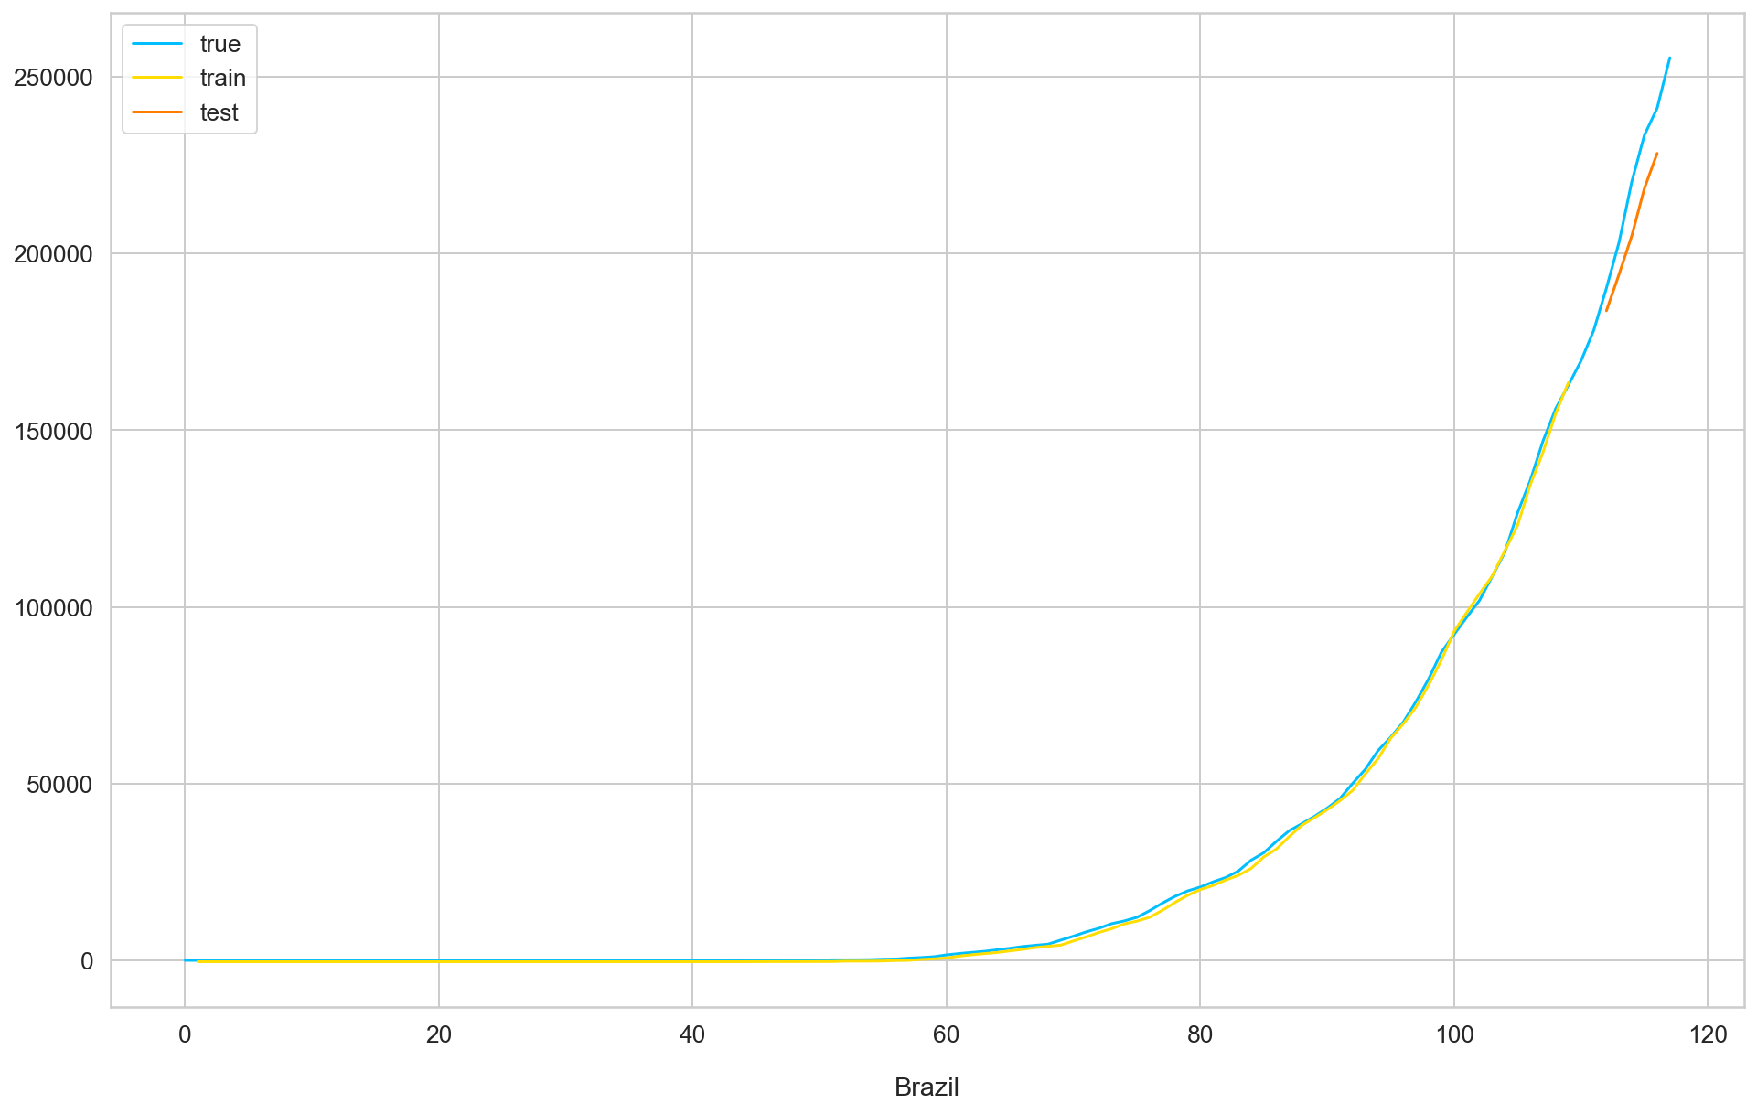
\includegraphics[width=4.8cm]{Brazil_LSTM.pdf}
		\end{minipage}
	}
	\subfigure[德国] {
		\begin{minipage}{0.3\linewidth}
			\centering
			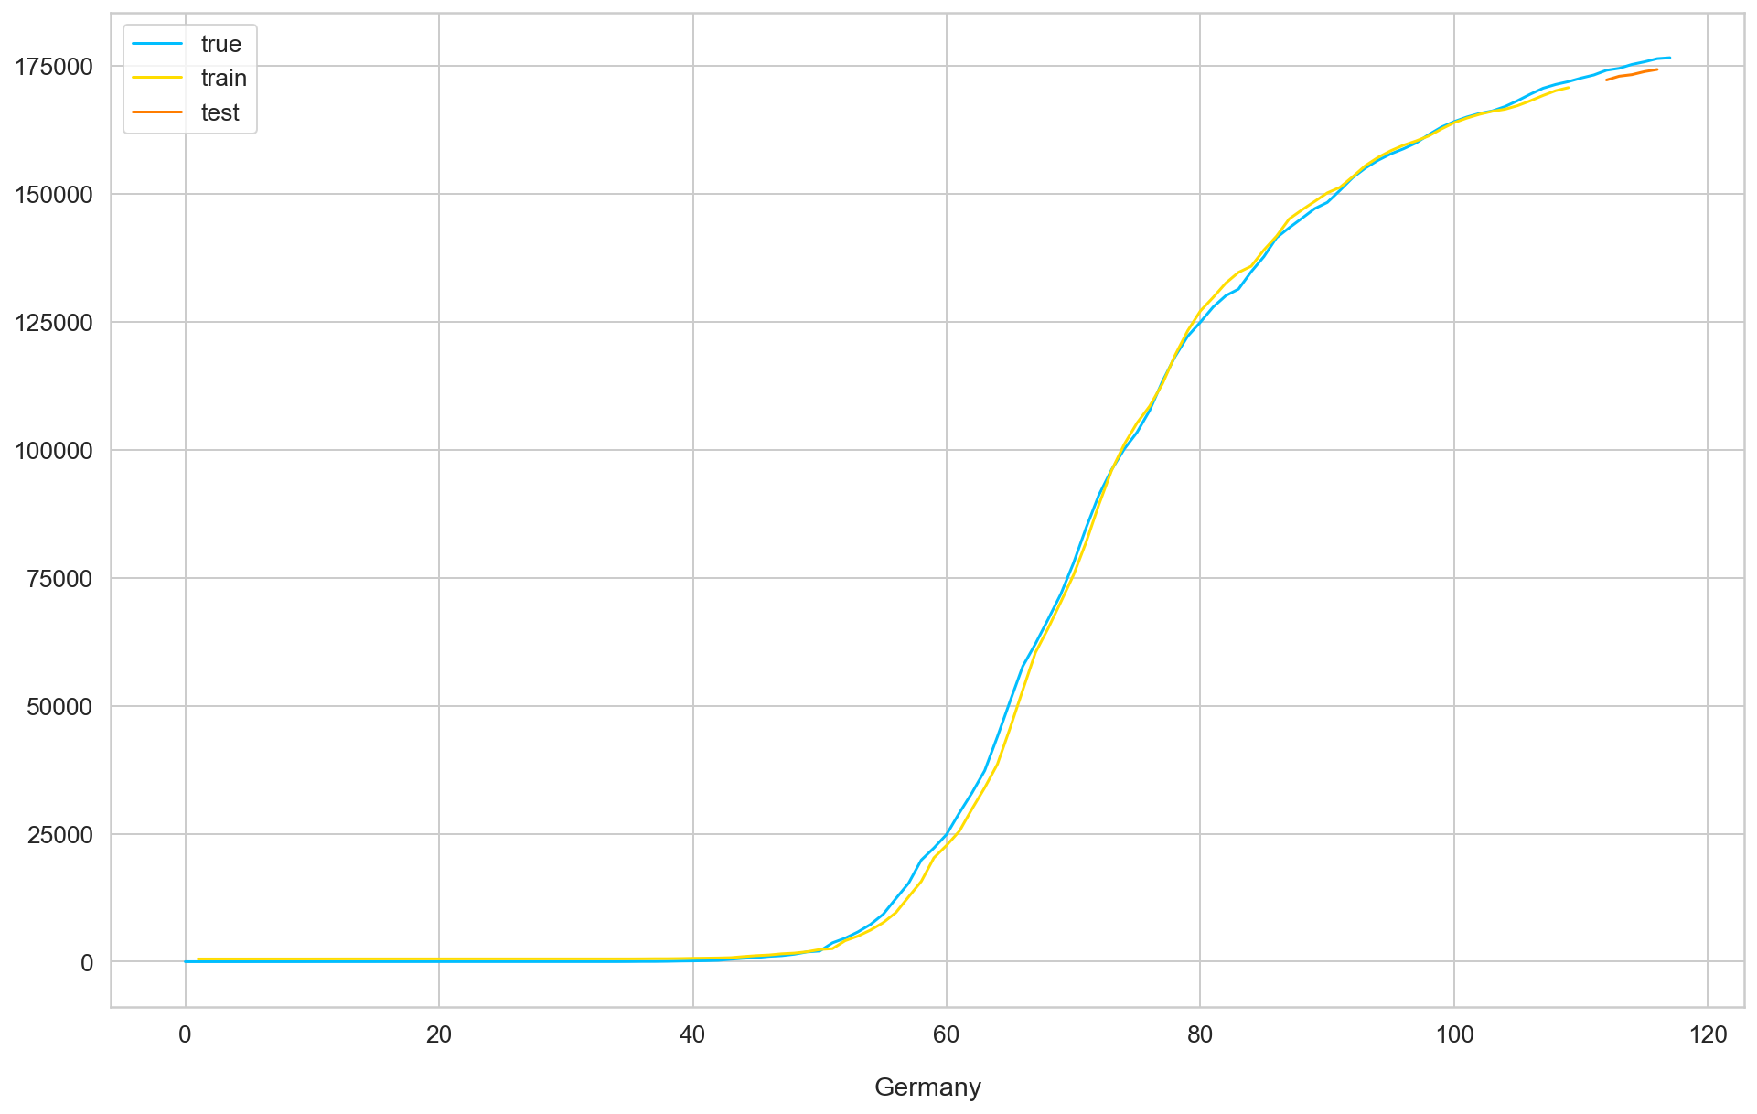
\includegraphics[width=4.8cm]{Germany_LSTM.pdf}
		\end{minipage}
	}
	\subfigure[意大利] {
		\begin{minipage}{0.3\linewidth}
			\centering
			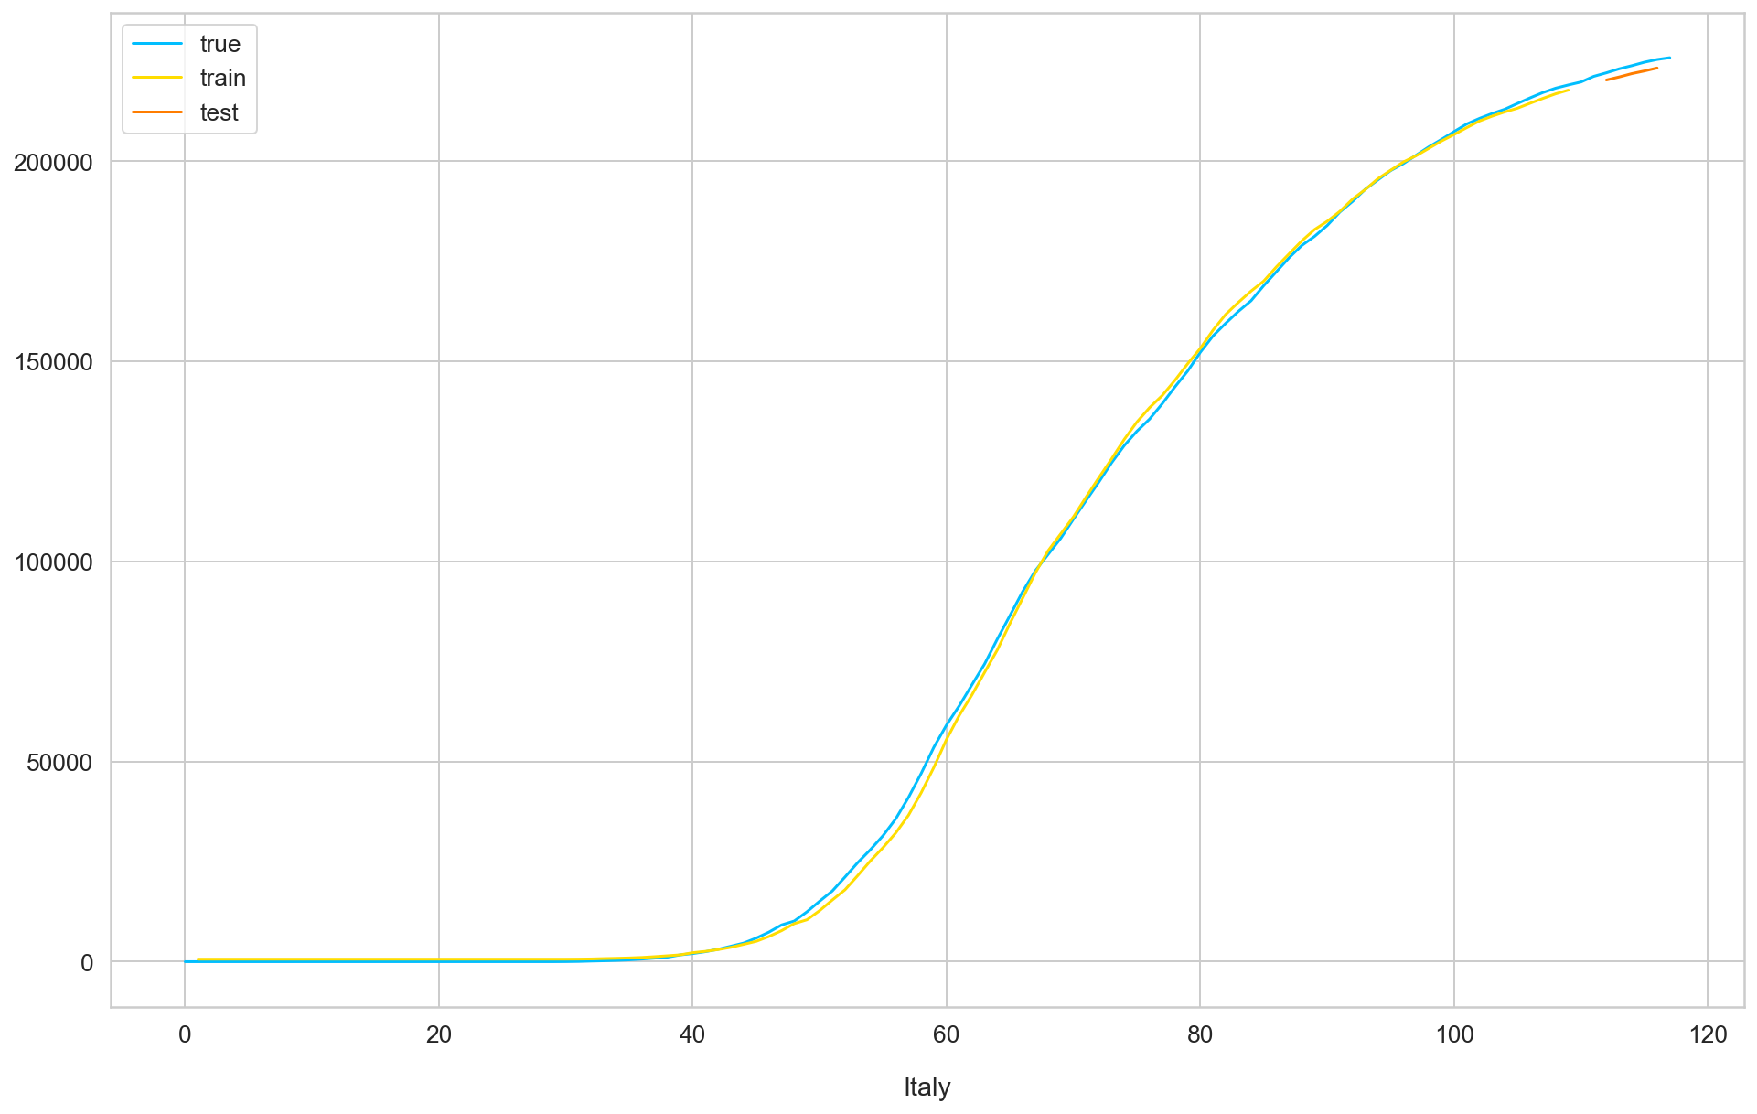
\includegraphics[width=4.8cm]{Italy_LSTM.pdf}
		\end{minipage}
	}
	\\
	\subfigure[俄罗斯] {
		\begin{minipage}{0.3\linewidth}
			\centering
			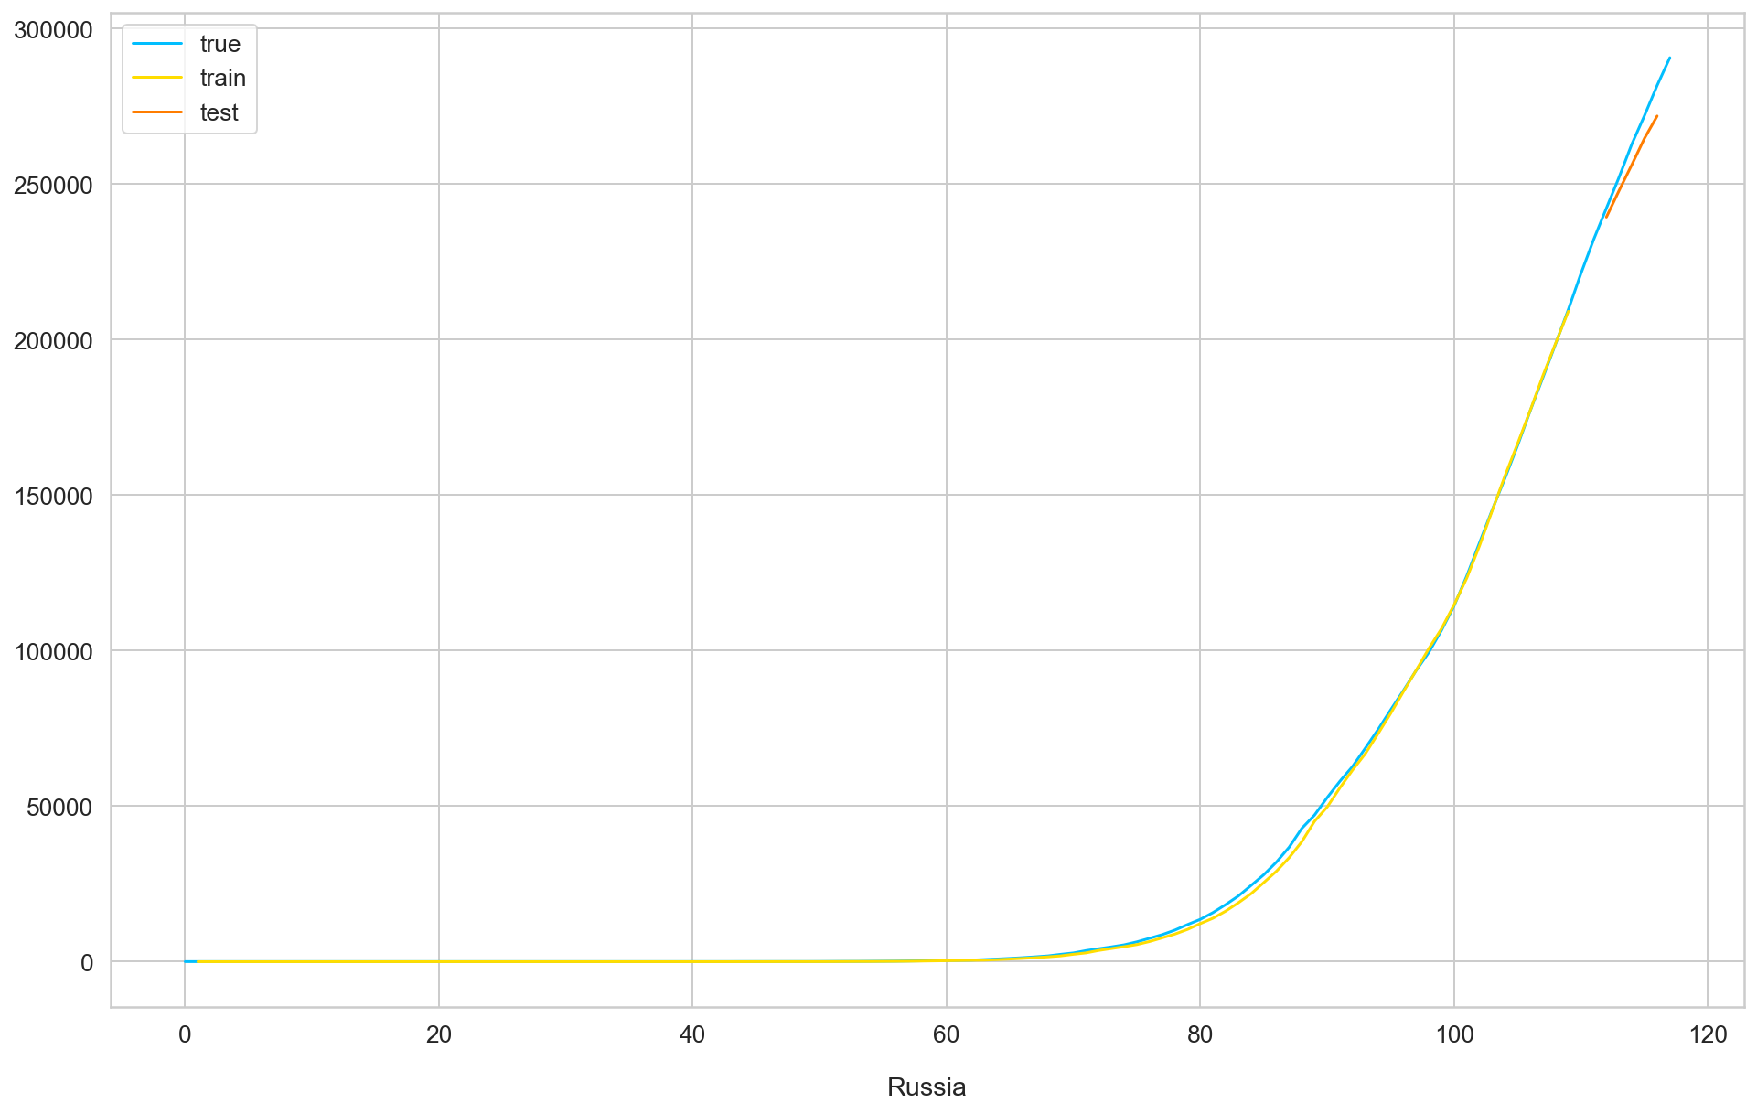
\includegraphics[width=4.8cm]{Russia_LSTM.pdf}
		\end{minipage}
	}
	\subfigure[英国] {
		\begin{minipage}{0.3\linewidth}
			\centering
			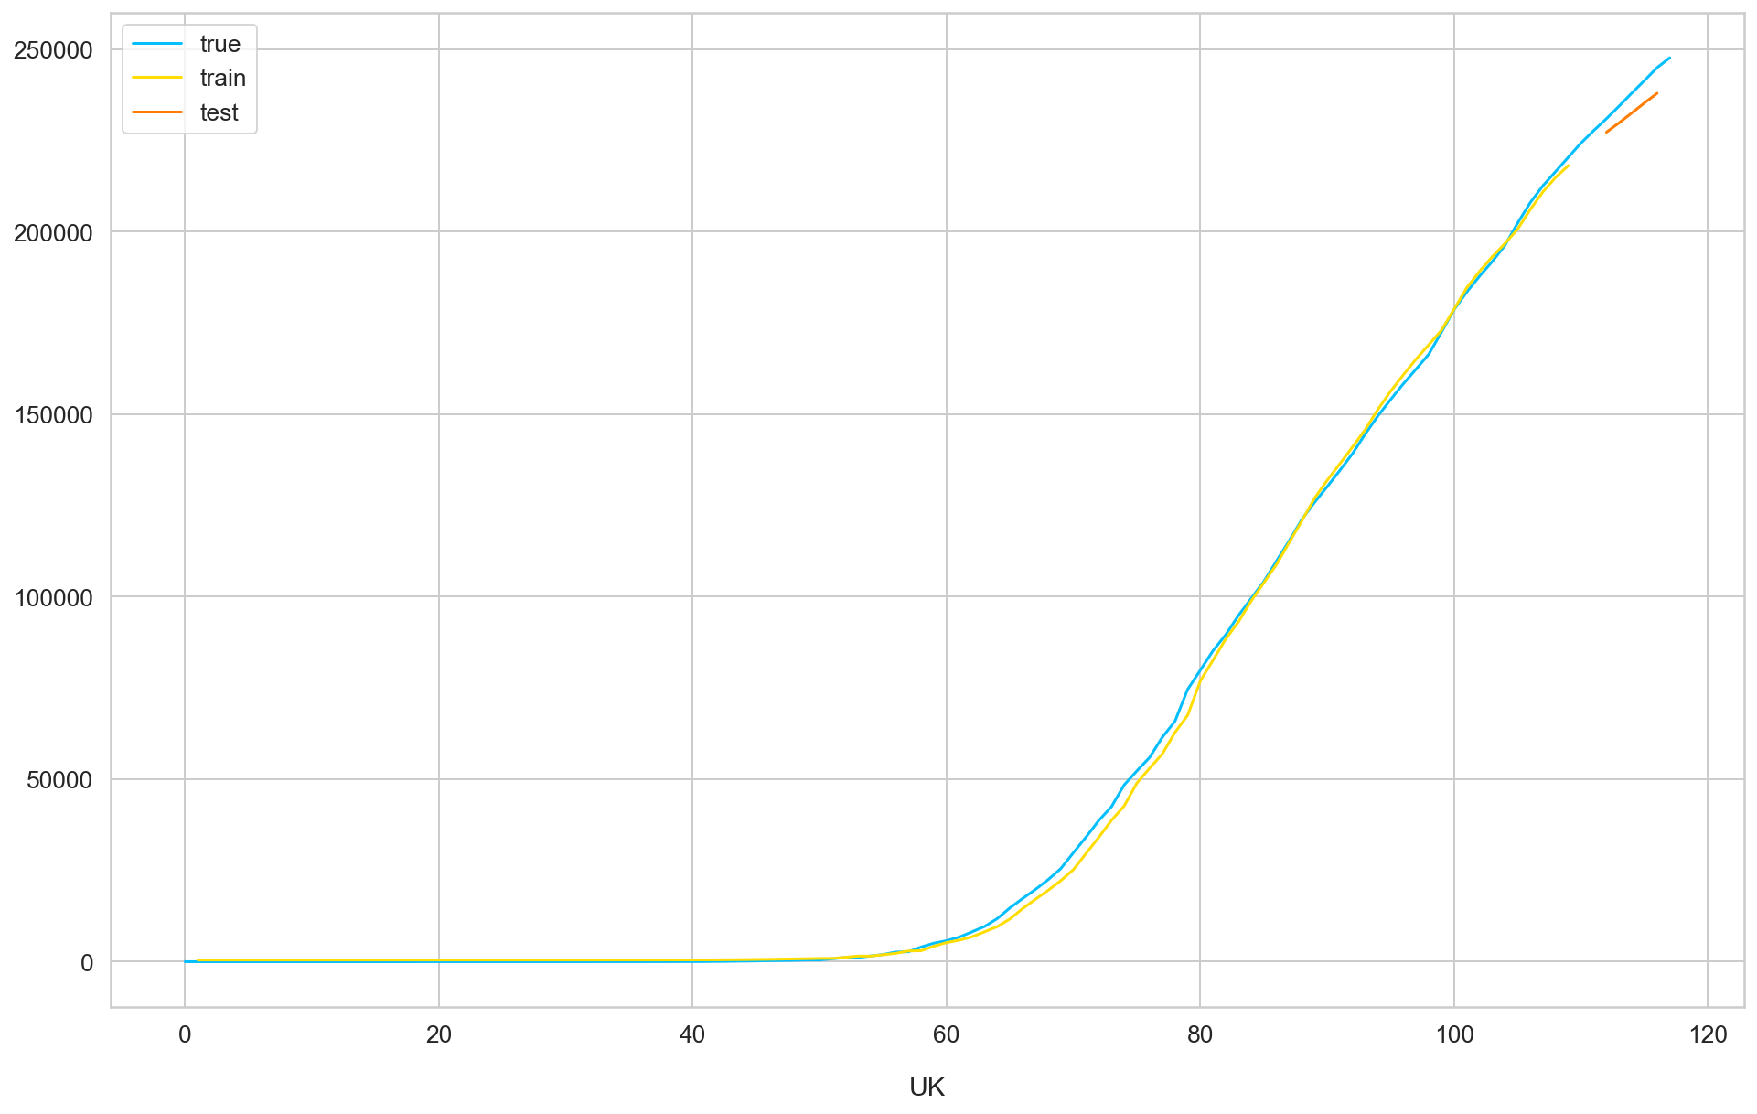
\includegraphics[width=4.8cm]{UK_LSTM.pdf}
		\end{minipage}
	}
	\subfigure[美国] {
		\begin{minipage}{0.3\linewidth}
			\centering
			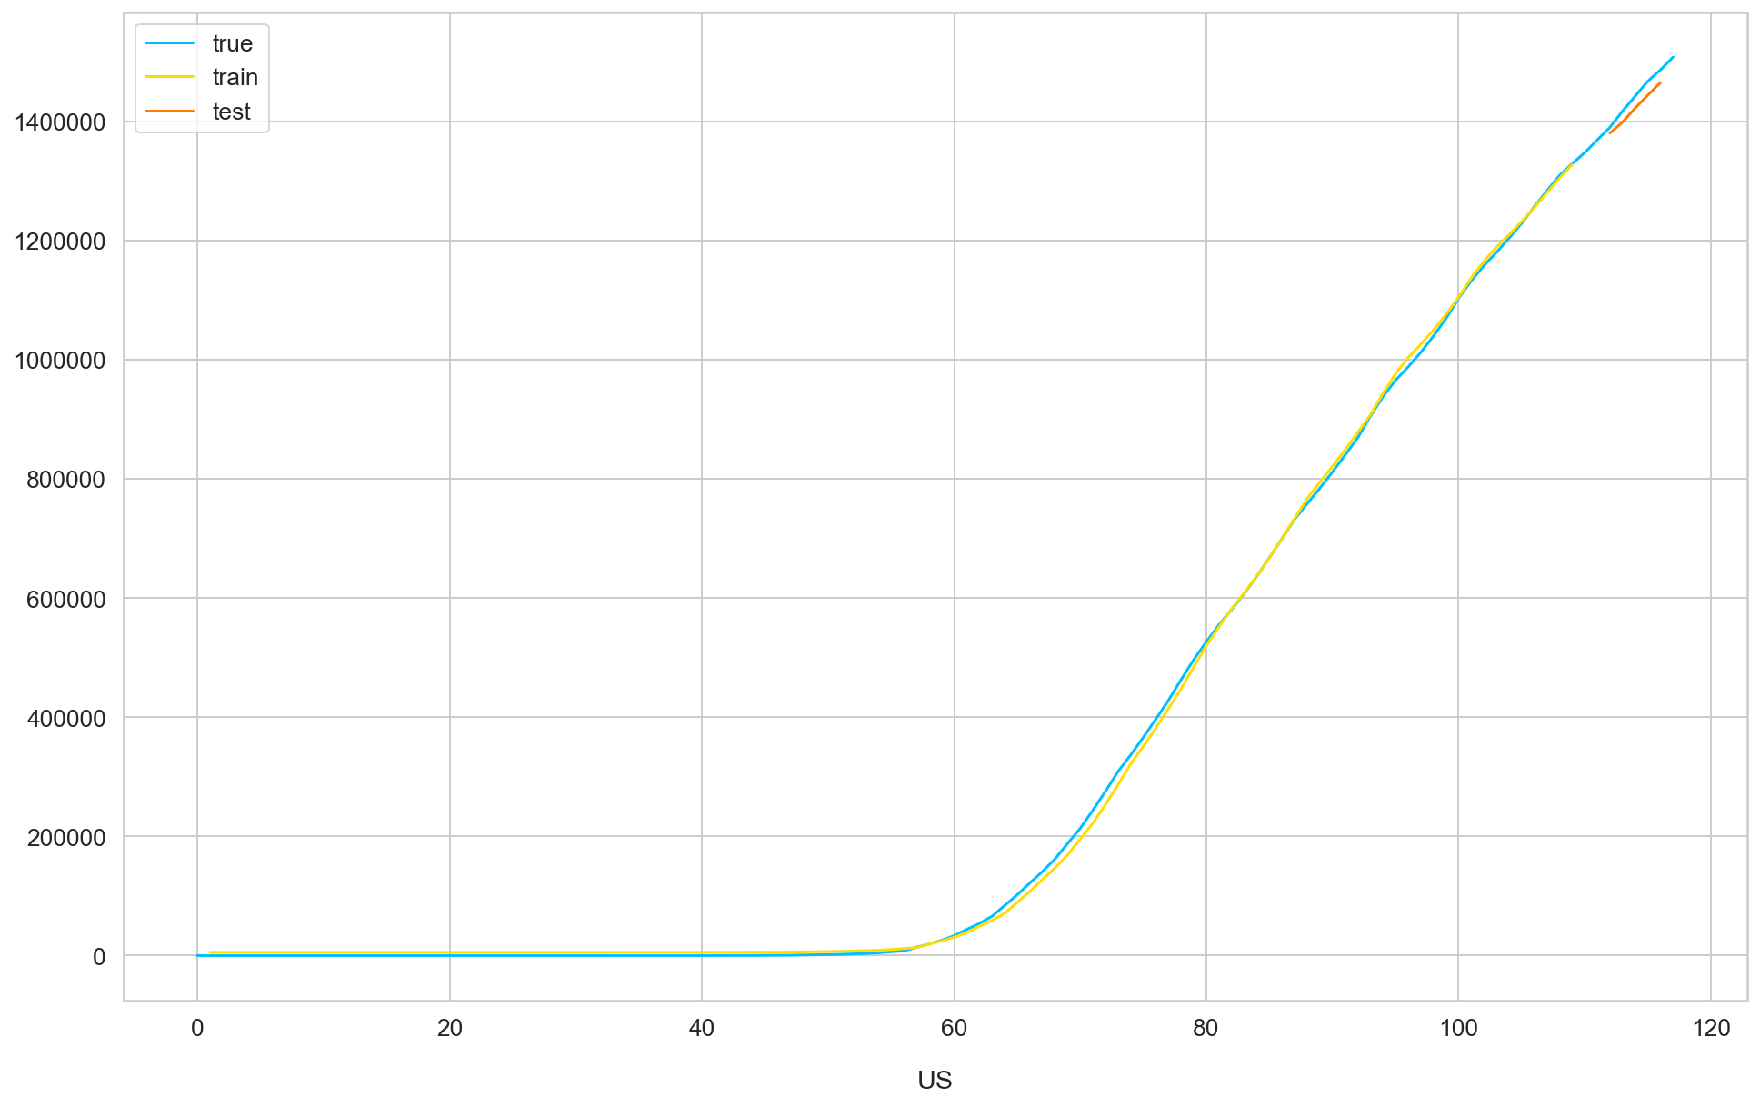
\includegraphics[width=4.8cm]{US_LSTM.pdf}
		\end{minipage}
	}
	\caption{LSTM模型的模拟}
	\label{fig:LSTMfit}
\end{figure}

\subsection{SEIR与LSTM的模型预测}

将2020年1月22日至2020年5月18日的疫情数据作为训练集,分别使用SEIR模型和LSTM模型预测5月19
日至5月24日巴西、德国、意大利、俄罗斯、英国和美国的COVID-19累计确诊人数,并比较它们的RMSE
损失。如表\ref{table:score}所示,LSTM模型的RMSE远小于SEIR模型。

\begin{table}[htp]
	\centering
	\caption{六个国家的预测RMSE损失比较}
	\label{table:score}
	\begin{tabular}{cccccccc}
		\hline
		& 巴西 & 德国 & 意大利 & 俄罗斯 & 英国 & 美国 \\
		\hline
		SEIR & 15498478 & 4315 & 3905940 & 19031588 & 1082278 & 10278735 \\
		LSTM & 12229.01 & 1905.93 & 2031.12 & 6644.43 & 5508.75 & 19200.5 \\
		\hline
	\end{tabular}
\end{table}

分别使用SEIR模型和LSTM模型对未来5天的全球COVID-19累计确诊人数进行预测,这是因为考虑所
有国家/地区的数据,使得模型提取更多的信息,从而使得模型的准确度更高。

\begin{table}[htp]
	\centering
	\caption{全球确诊人数预测}
	\label{table:pred}
	\begin{tabular}{cccccc}
		\hline
		& 05/25 & 05/26 & 05/27 & 05/28 & 05/29 \\
		\hline
		SEIR & 106816753 & 120811582 & 136419044 & 153760588 & 172947403 \\
		LSTM & 4897492 & 4996472 & 5102424 & 5210817 & 5310362 \\
		\hline
	\end{tabular}
\end{table}

\section{讨论}

从数理模型的角度来看,SEIR模型是用来估计传染病的,而LSTM模型则运用于时间序列预测分析。
与SEIR模型相比,LSTM模型可以更好地拟合已有数据,因为它是经过现有数据训练的,但是无法准
确地判断和融合传染特征。因此认为LSTM模型更适用于短期内预测。另一方面,SEIR模型通过考虑
多人群的相互作用和关联,引入了更多的变量和因素,更符合传染病发展规律,但是在考虑不同的干
预措施时,预测结果会有很大差异。

本文存在一些局限性。数理模型通过快速合并多个输入以产生预测结果。但是,这一过程涉及到对不
确定因素的假设,例如,很难准确地确定人们遵守当地政府的检疫政策或措施的程度,以及可能影响
实际接触率和随后的接触率的公共行为,如洗手、带口罩、社交距离等。这些模型也缺乏足够的数据
来估计特定人群的隔离比例。实际上,传染病的演变是相当复杂的,我们的研究只考虑了最经典的SEIR
模型,并未对其进行展开,对于LSTM模型,没有考虑隐藏层数目、迭代次数等参数对模型的影响。此
外,还有许多未考虑的因素,例如病毒的传播方式、人口特征、自然环境等,例如空气污染可能会加
快病毒的传播。各国对病毒的检测率、在医疗资源(例如测试套件和进行测试的医疗专业人员)的数量
和质量上也有所不同。

\bibliography{report}

\end{document}
